\documentclass[12pt,a4paper,bibliography=totocnumbered,listof=totocnumbered]{scrartcl}
%\documentclass[12pt,a4paper]{article}
\usepackage[ngerman]{babel}
\usepackage[utf8]{inputenc}
\usepackage{amsmath}
\usepackage{amsfonts}
\usepackage{amssymb}
\usepackage{graphicx}
\usepackage{fancyhdr}
\usepackage{tabularx}
\usepackage{geometry}
\usepackage{setspace}
\usepackage[right]{eurosym}
\usepackage[printonlyused]{acronym}
\usepackage{subfig}
\usepackage{floatflt}
\usepackage[usenames,dvipsnames]{color}
\usepackage{colortbl}
\usepackage{paralist}
\usepackage{array}
\usepackage{titlesec}
\usepackage{parskip}
\usepackage[right]{eurosym}
\usepackage[subfigure,titles]{tocloft}
\usepackage[pdfpagelabels=true]{hyperref}

\usepackage{listings}
\lstset{basicstyle=\footnotesize, captionpos=b, breaklines=true, showstringspaces=false, tabsize=2, frame=lines, numbers=left, numberstyle=\tiny, xleftmargin=2em, framexleftmargin=2em}
\makeatletter
\def\l@lstlisting#1#2{\@dottedtocline{1}{0em}{1em}{\hspace{1,5em} Lst. #1}{#2}}
\makeatother

\geometry{a4paper, top=27mm, left=20mm, right=20mm, bottom=35mm, headsep=10mm, footskip=12mm}


\hypersetup{unicode=false, pdftoolbar=true, pdfmenubar=true, pdffitwindow=false, pdfstartview={FitH},
	pdftitle={Wahlpflichtfach: Projekt: Client-K.I.s (ReversiXT, SS \the\year)},
	pdfauthor={Dr.\ Carsten Kern},
	pdfsubject={Projektbericht},
	pdfcreator={\LaTeX\ with package \flqq hyperref\frqq},
	pdfproducer={pdfTeX \the\pdftexversion.\pdftexrevision},
	pdfkeywords={Projektbericht, ReversiXT},
	pdfnewwindow=true,
	colorlinks=true,linkcolor=black,citecolor=black,filecolor=magenta,urlcolor=black}
\pdfinfo{/CreationDate (D:20151500000000)}
\titlespacing{\section}{0pt}{12pt plus 4pt minus 2pt}{-6pt plus 2pt minus 2pt}

% Kopf- und Fusszeile
\renewcommand{\sectionmark}[1]{\markright{#1}}
\renewcommand{\leftmark}{\rightmark}
\pagestyle{fancy}
\lhead{}
\chead{}
\rhead{\thesection\space\contentsname}
\lfoot{Implementierung von Brettspielen am Beispiel ReversiXT -- SS \the\year}
\cfoot{}
\rfoot{\ \linebreak Seite \thepage}
\renewcommand{\headrulewidth}{0.4pt}
\renewcommand{\footrulewidth}{0.4pt}

% Vorspann
\renewcommand{\thesection}{\Roman{section}}
\renewcommand{\theHsection}{\Roman{section}}
\pagenumbering{Roman}

\newcommand{\folgen}[1]{
\ensuremath
#1
}

\newcommand{\MyTitlepage}[5][\empty]{
\thispagestyle{empty}
\begin{center}
	
\includegraphics[scale=0.2]{pics/oth-logo.png}\\
	\vspace*{2cm}
	\Large
	\textbf{Fakultät}\\
	\textbf{Informatik und Mathematik}\\
	\vspace*{2cm}
	\Huge
	\textbf{Projektbericht}\\
	\vspace*{0.5cm}
	\large
	zum Wahlpflichtfach im SS \the\year\\
	\vspace*{1cm}
	\textbf{Projekt: Client-K.I.s (ReversiXT)}\\
	\vspace*{1cm}
	\includegraphics[height=6cm]{#1}
	\vfill
	\normalsize
	%\newcolumntype{x}[1]{>{\raggedleft\arraybackslash\hspace{0pt}}p{#1}}
	\begin{tabular}{rl}%{6cm}p{7.5cm}}
	    \rule{0mm}{5ex}\textbf{Gruppe:} & #2 \\
		\rule{0mm}{5ex}\textbf{Autoren:} & \hspace*{-0.5em}\begin{tabular}[t]{r}#3\end{tabular} \\ 
		\rule{0mm}{5ex}\textbf{Leiter:} & Prof. Dr. rer. nat. Carsten Kern \\ 
		\rule{0mm}{5ex}\textbf{Abgabedatum:} & #4 \\ 
	\end{tabular} 
\end{center}
\pagebreak
}
\usepackage{graphicx}
\usepackage{wrapfig}

\begin{document}


    % ----------------------------------------------------------------------------------------------------------
    % Titelseite
    % ----------------------------------------------------------------------------------------------------------
    \MyTitlepage[pics/Titelbild.png]{07}{
    \texttt{Katharina.Greim@st.oth-regensburg.de}\\
    \texttt{Florian.Klamer@st.oth-regensburg.de}\\
    \texttt{Tim.Lechner@st.oth-regensburg.de}}
    {05.07.\the\year} % FIXME optional: Gruppenlogo als PNG, Pflichtfelder: Gruppe, Authoren durch "\\" getrennt und Abgabedatum eingeben

    \setcounter{page}{1}
    % ----------------------------------------------------------------------------------------------------------
    % Inhaltsverzeichnis
    % ----------------------------------------------------------------------------------------------------------
    \tableofcontents
    \pagebreak


    % ----------------------------------------------------------------------------------------------------------
    % Inhalt
    % ----------------------------------------------------------------------------------------------------------
    % Abstände Überschrift
    \titlespacing{\section}{0pt}{12pt plus 4pt minus 2pt}{-6pt plus 2pt minus 2pt}
    \titlespacing{\subsection}{0pt}{12pt plus 4pt minus 2pt}{-6pt plus 2pt minus 2pt}
    \titlespacing{\subsubsection}{0pt}{12pt plus 4pt minus 2pt}{-6pt plus 2pt minus 2pt}

    % Kopfzeile
    \renewcommand{\sectionmark}[1]{\markright{#1}}
    \renewcommand{\subsectionmark}[1]{}
    \renewcommand{\subsubsectionmark}[1]{}
    \lhead{Kapitel \thesection}
    \rhead{\rightmark}

    \onehalfspacing
    \renewcommand{\thesection}{\arabic{section}}
    \renewcommand{\theHsection}{\arabic{section}}
    \setcounter{section}{0}
    \pagenumbering{arabic}
    \setcounter{page}{1}

    % ----------------------------------------------------------------------------------
    % Kapitel: Einleitung
    % ----------------------------------------------------------------------------------
    \section{Einleitung}
    \vspace{1em}

    %Leiten Sie in diesem Abschnitt in das Fach YIMB und das zu erstellende Projekt ein. %Beschreiben Sie kurz die Fragestellung, die in diesem Wahlpflichtfach gelöst werden %soll. Stellen Sie Ihr vorhandenes Vorwissen dar, das in dieser Veranstaltung für Sie %von Nutzen sein könnte/ist/war, etc.
		
    Dieses Projekt basiert auf Reversi, ein ca. 100 Jahre altes Brettspiel. Ursprünglich ist es ein Spiel, bei dem zwei Spieler auf einem 8x8 großen Spielfeld um den Sieg fechten. Durch abwechselndes Legen von Spielsteinen versucht man so viel Fläche wie möglich zu besetzten. Der Kniff dabei ist, dass vom Gegner eingefärbte Felder durch geschicktes platzieren eigener Steine wieder invertiert werden können, daher auch der Name Reversi. Abbildung \ref{fig:Reversi} zeigt das typische Spielfeld. In der Mitte liegen die Steine der zwei Spieler in der Startposition.
    
    \vspace{1em}
    \begin{minipage}{\linewidth}
    	\centering
    	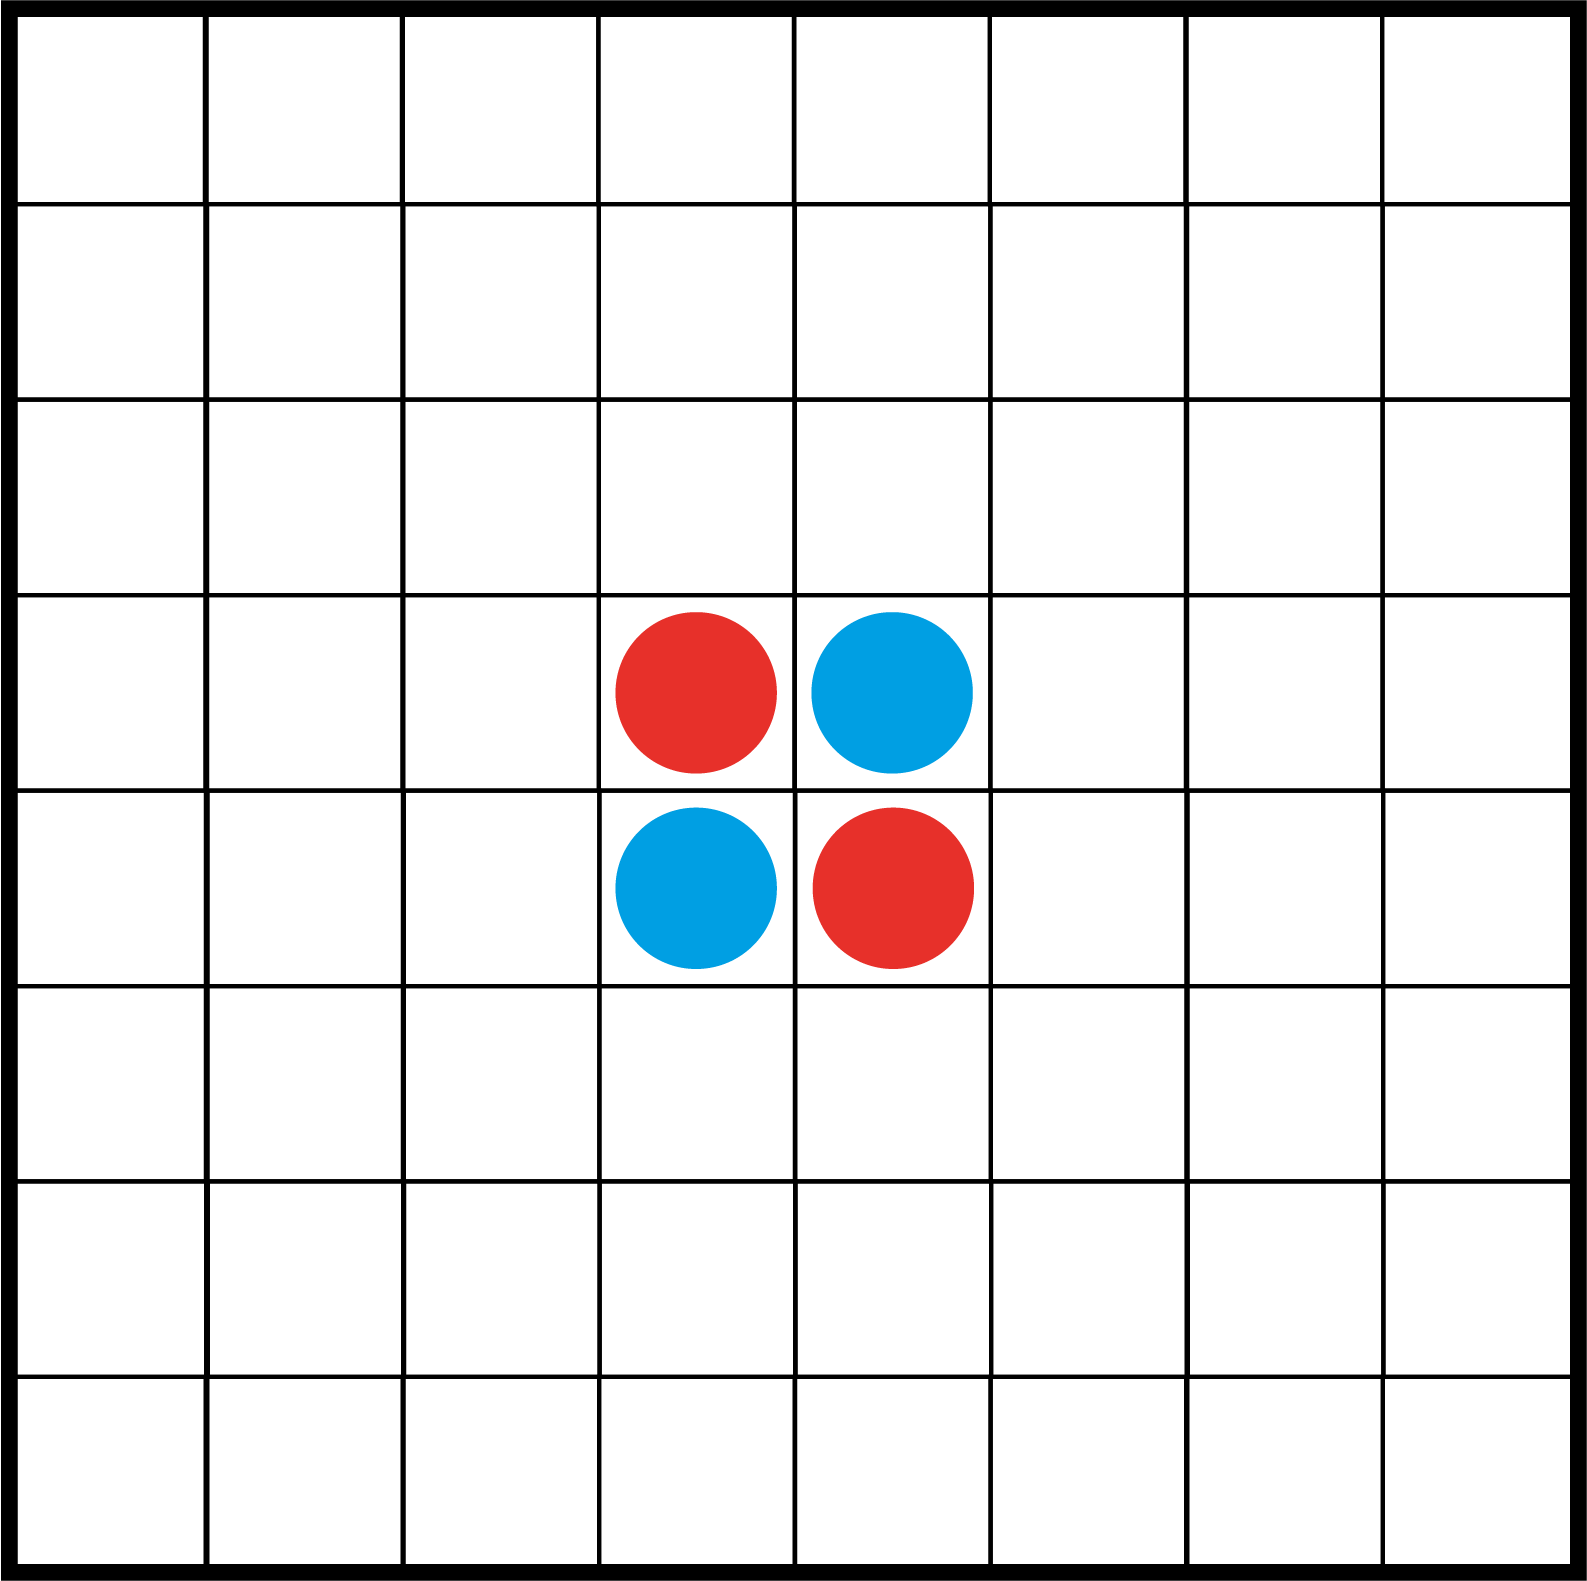
\includegraphics[width=0.6\linewidth]{pics/Kapitel_1/Kapitel_1_pic1.png}
    	\captionof{figure}[Reversi]{\glqq Standard\grqq{} Reversi }
    	\label{fig:Reversi}
    \end{minipage}
    \vspace{1em}
    
    Wie anfangs schon erwähnt, hat die Standardversion von Reversi ein relativ kleines Spielfeld und nur zwei Spieler. Es gibt nur zwei Arten von Spielsteinen, nämlich die der zwei Spieler Das steht im starken Kontrast zu ReversiXT, für das dieses Projekt eine KI entwickelt. Abbildung \ref{fig:ReversiXT} zeigt die meisten, der nun genannten Features von ReversiXT. In der erweiterten Version des Spiels, sind bis zu acht Spieler erlaubt. Um verschiedene Teile der Karte zu verbinden, gibt es Transitionen, die wie \glqq Portale \grqq{} funktionieren (gelbe Linien auf Abb. \ref{fig:ReversiXT}). Spieler können durch diese, in die ausgehende Richtung, das Zielfeld über die dortige Richtung färben. Dadurch wird das Spielfeld nochmal komplexer und für den Menschen schwerer zu überblicken.  Außerdem gibt einige Sonder-Spielsteine und Felder. Diese Steine bestehen aus \glqq Überschreibsteinen\grqq, die es ermöglichen gegnerische Spielsteine umzufärben und \glqq Bomben\grqq. Mit diesen kann man in der zweiten Phase des Spiels Bereiche des Spielbretts zerstören. Dazu folgt später mehr. Die neuen Spielfelder sind \glqq Wahlfeld\grqq{} oder \glqq choise \grqq{} (hellgrünes Feld mit großem C auf Abb. \ref{fig:ReversiXT}), welches es dem besetzenden Spieler ermöglicht, mit einem Mitspieler seiner Wahl Spielsteine zu tauschen (auch mit sich selbst). \glqq Inversionsfelder\grqq, wenn besetzt, verschieben die Spielerfarben um eins. Besetzt ein Spieler ein \glqq Bonusfeld\grqq (oranges Feld mit großem B auf Abb. \ref{fig:ReversiXT}) so hat er die Möglichkeit eine extra Bombe oder einen extra Überschreibstein zu erhalten. Zuletzt gibt es noch \glqq Expansionsfelder\grqq (graues Feld mit großem X auf Abb. \ref{fig:ReversiXT}). Diese agieren wie \glqq tote\grqq{} Spieler und können durch normale Züge oder das Platzieren von Überschreibsteinen eingefärbt werden. Zuletzt gilt es noch die leeren Felder oder auch \glqq Löcher \grqq{} genannten Felder zu erwähnen (auf Abb. \ref{fig:ReversiXT} als dunkelgraue Felder zu erkennen). Diese verhalten sich wie der Spielfeldrand und man kann nicht auf sie ziehen.
    
    \vspace{1em}
    \begin{minipage}{\linewidth}
    	\centering
    	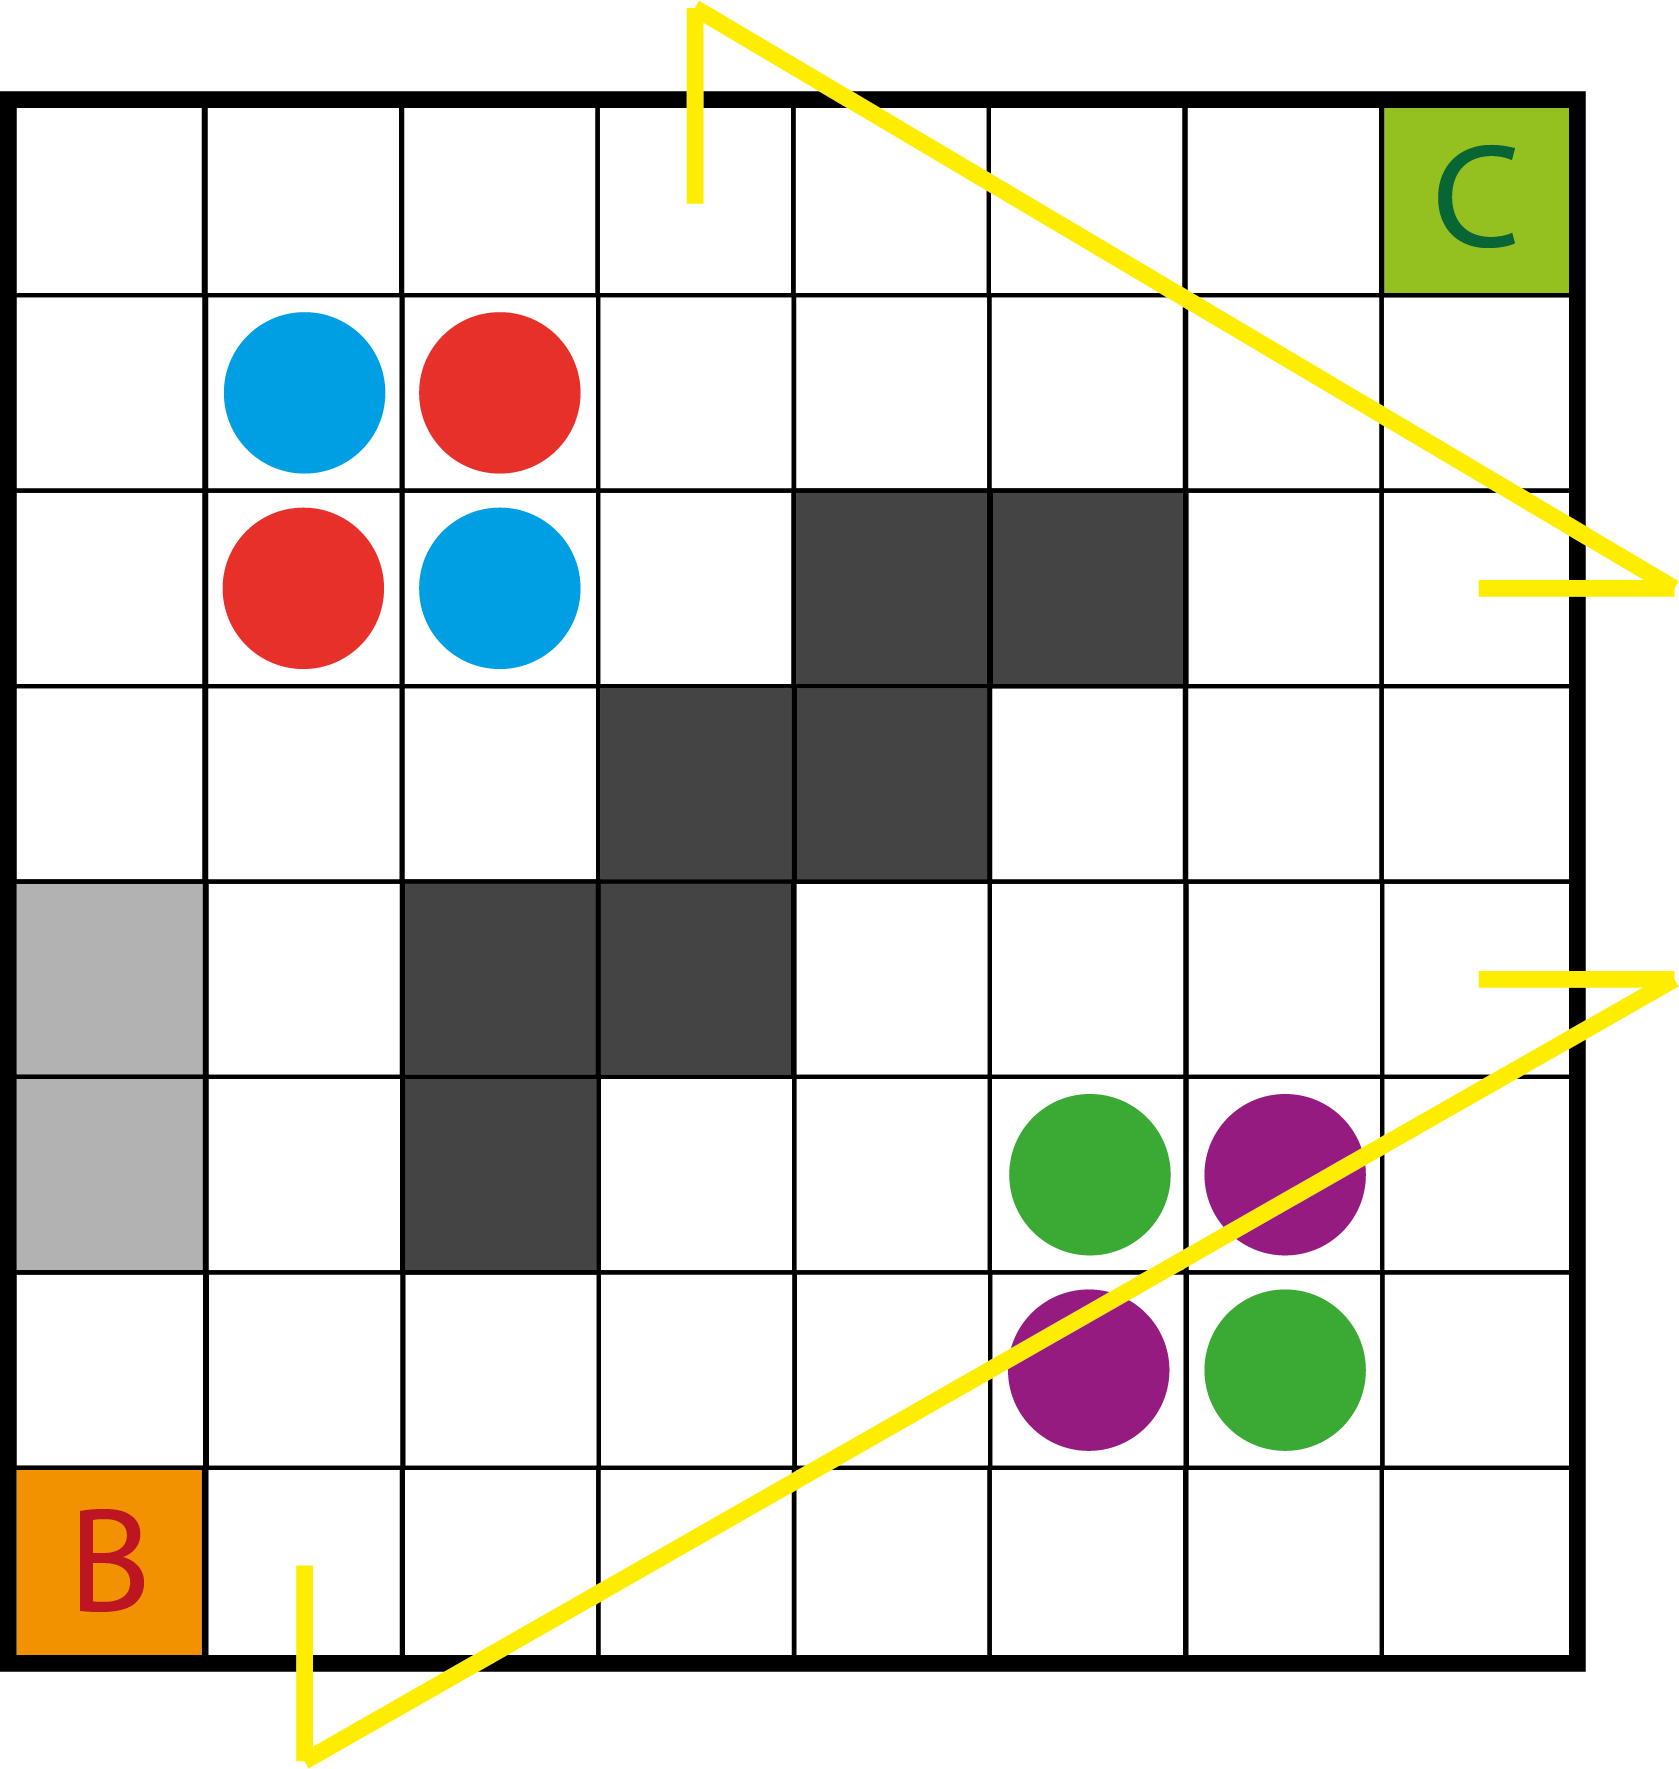
\includegraphics[width=0.6\linewidth]{pics/Kapitel_1/Kapitel_1_pic2.png}
    	\captionof{figure}[ReversiXT]{ReversiXT mit neuen Features}
    	\label{fig:ReversiXT}
    \end{minipage}
   	\vspace{1em}

    Unsere Aufgabe in diesem Projekt ist es, einen künstlichen-Intelligenz Spieler Clienten zu programmieren. Dieser soll gegen andere KIs auf einem, von einem Server gehostetem Spiel antreten. Grundvoraussetzung ist natürlich, dass die KI nur gültige Züge berechnet und einer von uns entwickelten Heuristik folgt. Diese Heuristik ist das Herzstück des Projekts. Sie ist maßgeblich dafür verantwortlich, gute Zugentscheidungen zu treffen und schließlich das Spiel zu gewinnen. All die oben genannten Schritten sind Vorbereitung für einen großen Wettkampf gegen Ende des Semesters. In der Endphase des Wahlpflichtmoduls findet nämlich ein virtueller Wettstreit zwischen den KIs der Studenten der RWTH Aachen und der OTH Regensburg statt. Historisch ist die OTH schon oft als Sieger hervorgegangen und wir hoffen auch dieses Jahr auf einen Sieg.

    Insgesamt sieht unser Team dieses Projekt als gute Lernmöglichkeit um unsere Programmier-, Team- und weitere Fähigkeiten zu erweitern. Wir kommen alle mit relativ wenig Erfahrung in dieses Projekt und hoffen deswegen, die oben genannten und viele weitere Dinge zu vertiefen.

    % ----------------------------------------------------------------------------------
    % Kapitel: Allgemeine Informationen
    % ----------------------------------------------------------------------------------
    \section{Allgemeine Informationen}
    \vspace{1em}

    In diesem Teil werden die technischen und sozialen Rahmenbedingungen des Projekts erläutert und weitere allgemeine Informationen dargelegt. Das soll helfen, das Projekt und alle Beteiligten daran in Perspektive zu setzten. Außerdem können so Entscheidungen über verwendete Technologien aus Sicht des Teams besser nachvollziehbar gemacht werden. Die Vorstellung des Teams eröffnet dieses Kapitel und wird gefolgt von der Beschreibungen der eingesetzten Software sowie der verwendeten Datenstruktur die zur Speicherung des Spielfeldes und verbundenen Daten dient.

    \subsection{Team und Kommunikation}
    \vspace{1em}
    %Beschreiben Sie in diesem Abschnitt Ihr Team. Welche Person hat welche Aufgaben %wahrgenommen, wie wurden Aufgaben aufgeteilt und wie wurde kommuniziert, etc.
    Alle aus dem Team befinden sich gerade im 4. Semester der allgemeinen Informatik. Daher kennen wir uns bereits aus den letzten Semestern uns sehen uns häufig in den Vorlesungen, wodurch ein Großteil der Kommunikation im Team bereits dort stattfindet. Zusätzlich stehen wir über Whats-App, die Gruppenmailingliste und über das lokale Gruppen-Repository in Kontakt.

    Obwohl das Team im gleichen Studiengang ist hat jedes Teammitglied natürlich einen eigenen Werdegang und damit auch andere Erfahrungen und Fähigkeiten. Diese werden in diesem Abschnitt nun im Zusammenhang zum Projekt erläutert.

	%TODO Kathi genauer erklären was für fähigkeiten für was im konkret wichtig waren
    Katharina Greim hat in den ersten drei Semestern ihres Studiums Programmierkenntnisse in Java und C erlernt. In den Vorlesungen Mathematik 1 \& 2 und Algorithmen \& Datenstrukturen wurde das Lösen von abstrakten Problemen und Implementieren von verschiedenen Datenstrukturen oft geübt. Da Sie zusätzlich ein Tutorium hält, hat sie gelernt, individuell auf Menschen einzugehen und komplizierte Dinge leicht verständlich zu erklären, was bei der Arbeit im Team sehr hilfreich sein wird. Außerdem hat sie bereits einige Erfahrungen mit \LaTeX\quad gesammelt.

    Florian Klamer hat Vorkenntnisse aus früheren Vorlesungen wie Programmieren 1 \& 2 die grundsätzlich wichtig für die Implementierung und Strukturierung der KI sind. Aus Algorithmen und Datenstrukturen sind die Teile wichtig, bei denen es um effiziente und sichere Algorithmen für z.B die Berechnung der Heuristik oder der gültigen Züge geht. Neben dem Studium hilft Florian außerdem ehrenamtlich beim Connecta e.V. mit. Dort ist er im EDV Ressort mit der Betreuung des Intra-, Extranets, der Datenbank und der Webseite beschäftigt. Die dort erworbenen Fähigkeiten sind z.B. in Git, SQL oder Teamarbeit, können aber ebenso wichtig für das Projekt sein.

    Tim Lechner hat die für das Projekt erforderlichen Vorkenntnisse aus früheren Vorlesungen wie Programmieren 1 \& 2, Algorithmen und Datenstrukturen erworben. 
    

    Der letzte Teil in diesem Abschnitt ist eine Liste (Tabelle 1) der Übungsaufgaben und von wem sie bearbeitet wurden.

    %TODO Tabelle vervollständigen und richtig plazieren
    \begin{table}[]
        \centering
        \caption{Aufgabenverteilung}
        \label{tab:Aufgabenverteilung}
        \begin{tabular}{|l|l|l|}
            \hline
            \textbf{Übung} & \textbf{Bearbeiter} & \textbf{Kommentar} \\ \hline
            1 & Alle   &       \\ \hline
            1.5 & Katharina   &           \\ \hline
            2.1 &  Katharina     &           \\ \hline
            2.2 &  Alle     &           \\ \hline
            2.3 &  Katharina     &           \\ \hline
            3.1 &    Florian   &           \\ \hline
            3.2 &    Florian   &           \\ \hline
            4.1 &      Tim &           \\ \hline
            4.2 &      Tim &           \\ \hline
            5 &      Katharina &           \\ \hline
            6.1 &    Katharina   &           \\ \hline
            6.2 &     Katharina  &           \\ \hline
            7.1 &     Katharina  &           \\ \hline
            7.2 &    Katharina   &           \\ \hline
            7.3 &    Florian   &           \\ \hline
            8.1 &    Florian   &           \\ \hline
            8.2 &    Tim, Katharina   &           \\ \hline
            8.3 &    Katharina   &           \\ \hline
            9.1 &     Katharina  &           \\ \hline
            9.2 &     Katharina  &           \\ \hline
            9.3 &      Katharina &           \\ \hline
            10.1 &    Katharina, Tim   &           \\ \hline
            10.2 &     Florian  &           \\ \hline
            11.1 &   Katharina    &           \\ \hline
            11.2 &   Katharina, Florian    &           \\ \hline
            11.3 &   Florian   &           \\ \hline
            12.1 &     Katharina, Tim  &           \\ \hline
            12.2 &    Alle   &           \\ \hline
        \end{tabular}
    \end{table}

    \subsection{Technische Daten}
    \vspace{1em}
    %Beschreiben Sie u.a.\ in welcher Programmiersprache und unter welchem Betriebssystem Sie entwickeln, welche IDEs Sie nutzen, welche zusätzlichen Tools bei Ihrer Projektentwicklung Einsatz gefunden haben, etc.
	%TODO Korrekturlesen
	%TODO eventuelle weitere Software eintagen
	Die Implementierung unseres Projekts berührt viele Bereiche wie z.B: Netzwerke, Heuristiken, Algorithmen, usw., weswegen verschiedenste Tools zum Programmieren und Testen nötig sind. Nun folgt die Beschreibung dieser und der verwendeten Hardware.
	
    Die Implementierung gestaltet unser Team mit Java 9. Das ist eine der Sprachen, die unser Team im Studium gelernt hat und am besten beherrscht. Als Betriebssystem verwenden wir alle hauptsächlich Windows 10. Manchmal, vor allem zum Testen, kommt auch Linux (Ubuntu)(Version 18.04) zum Einsatz. Im Team benutzen wir alle IntelliJ (Version 2018.1.3) von JetBrains. Diese IDE hat viele nützliche Features und ist für uns als Studenten für nicht kommerzielle Projekte kostenlos. Neben Git (2.18.0 64-Bit) verwenden wir Sourcetree (2.6.9 64-Bit) für eine übersichtliche Verwaltung und Sicherung unseres Quellcodes. Dieser Projektbericht ist mit dem Textsatzsystem LaTeX geschrieben. Hauptsächlich verwenden wir TeXstudio 2.12.8 als Editor, testen aber auch andere wie TeXworks, um die beste Arbeitsumgebung zu finden. Um Abbildungen für den Projektbericht zu gestalten verwenden wir Adobe Illustrator CC 22.1 64-Bit.\\
    Das letzte Tool zur Programmierung, ist das Buildtool Gradle (4.4). Es ist einfach zu benutzen und das Buildscript kann unter anderem, durch den Einsatz einer eigenen Sprache namens Groovy kurz und kompakt gestaltet werden. 

	Herr Kern hat uns freundlicherweise folgende, für unser Projekt zugeschnittene Programme, zu Verfügung gestellt.\\
    Um unser Programm gegen andere KIs testen zu können, verwenden wir den ReversiXT Server, der auch lokal Spiele hosten kann. Außerdem benutzen wir für den einfacheren Bau eigener Karten zur Verfügung gestellte Kartenbauprogramm.
    
    Zum Testen der KI und vor allem zum bestimmen möglichst optimaler Parameter zur Berechnung der Heuristik, haben wir eigene Bash-Skripte programmiert, die automatisch, viele Spiele auf verschiedenen Karten durchspielen. 

    Die Hardware auf denen wir programmieren und testen sind vor allem \glqq Mittelklasselaptops\grqq. Um den Rahmen nicht zu sprengen, sind hier die genauen Namen zu den Geräten aufgelistet, Details sind online zu finden.\\
    Florian benutzt ein Lenovo Yoga 720-15IKB-80X7.\footnotemark\\

    Tim setzt ein Lenovo ideapad Y700 ein.\footnotemark\\
    Katharina verwendet ein HP 250 G4 T6P08ES.\footnotemark\\

	
	
	\footnotetext{https://www.notebookcheck.com/Test-Lenovo-Yoga-720-15IKB-7700HQ-FHD-GTX-1050-Laptop.230060.0.html}
	\footnotetext{https://www.notebookcheck.com/Test-Lenovo-Ideapad-Y700-15ISK-80NW-Notebook.156295.0.html}
	
	\footnotetext{https://www.notebookcheck.com/Test-HP-250-G4-T6P08ES-Notebook.163379.0.html}
	
	


    \subsection{Datenstruktur}
    \vspace{1em}
    %Beschreiben Sie die Datenstruktur, die Sie zur Speicherung des Spielfeldes in Ihrem %Client nutzen. Gehen Sie auf Besonderheiten ein und erklären Sie, wie diese %funktionieren und was Sie sich davon erhoffen. Geben Sie falls möglich auch eine %schematische Darstellung/ein Bild der Datenstruktur an.
    Im ersten Versuch der Datenstruktur wurde die Anzahl der Spieler, Bomben, die Stärke usw. in Integer Variablen und das Spielfeld in einem String Array abgespeichert. Da diese Version viel Speicherplatz und Rechenzeit benötigt, wird sie ab sofort noch verbessert.
    Um die Datenstruktur zu verbessern, wollen wir folgende Punkte umsetzten:
    \newline
    1. Die Anzahl der Spieler, Überschreibsteine, Bomben sowie die Stärke der Bomben und die Spielfeldhöhe/-breite werden alle in Short Variablen gespeichert.

    Da die Anzahl der Spieler auf 8 begrenzt ist und auch das Spielfeld eine maximale Größe von 50 x 50 haben kann, reicht die Short Variable vollkommen aus. Auch für die Anzahl und Stärke der Bomben und Anzahl der Überschreibsteine wird die Größe eines Shorts genügen.

    2. Das Spielfeld wird in einem zweidimensionalem Charakter Array gespeichert.

    Da im Spielfeld nur einzelne Zeichen stehen, ist es sinnvoll einen Charakter und keinen String zu verwenden. Außerdem bietet sich ein Array sehr gut an, da die Höhe und Breite bereits vor dem Einlesen des Spielfeldes bekannt ist und somit sehr gut auf die einzelnen Felder zugegriffen werden kann.
    Eine zusätzliche Erweiterung wäre ein dreidimensionales Array, bei dem zu jedem Spielfeld noch zusätzliche Informationen abgespeichert werden können, z.B. ob eine Transition an dieser Stelle vorhaben ist.

    3. Die Transitionen werden so in einer Datenstruktur abgespeichert, dass eine schnelle Suche nach einer bestimmten Transition möglich ist.

    %TODO geeignete Datenstruktur für Transitionen nachtragen

    \newpage
    % ----------------------------------------------------------------------------------
    % Kapitel: Spielfeldbewertung
    % ----------------------------------------------------------------------------------
    \section{Spielfeldbewertung}
    \vspace{1em}
    Die Heuristik soll einen vorliegenden, beliebigen Spielstand für einen gegebenen Spieler bewerten. Das bedeutet, es soll ermittelt werden, ob dieser Zustand für den Spieler besonders gut oder schlecht ist. Somit können Züge später danach ausgesucht werden, ob eine Reihe von Zügen zu einer besonders guten Situation für einen Spieler oder auch zu einer besonders schlechten Situation für einen Gegenspieler führen kann.
    
    \subsection{Spielfeldbewertung: 1. Vorschlag}
    \vspace{1em}
    %Beschreiben Sie wie in der zugehörigen Projektaufgabe gefordert eine erste Heuristik.
	Die grundlegende Idee der ersten Spielfeldbewertung ist, Spielfelder anhand ihrer \glqq Färbbarkeit\grqq{} einzuschätzen. Als Hauptfaktor dient dazu wie schwer ein Feld vom Gegner umzufärben ist. Ist ein Feld z.B. nur noch von einer Seite einfärbbar, ist es sicherer als ein frei einfärbbares. Das bedeutet es bekommt eine bessere Bewertung. Wichtig ist außerdem die Beweglichkeit. Der Client soll das Spiel so lenken, dass er auf sicheren Steinen aufbauen kann, dabei aber nicht seine Mobilität, also die Anzahl an möglichen Zügen, verliert. In Summe führt das dazu, dass sich alle Spielsteine möglichst gegenseitig schützen.


    Um die Färbarkeit zu beurteilen, wird die Färbung in folgende vier Richtungen geprüft:

    1. horizontal - von links nach rechts oder umgekehrt \newline
    2. vertikal - von oben nach unten oder umgekehrt \newline
    3. von links oben nach rechts unten oder umgekehrt \newline
    4. von rechts oben nach links unten oder umgekehrt \newline


    \textbf{Beispiel 1:} Liegt ein Stein in einer Ecke, so ist es weder horizontal, vertikal oder schräg möglich diesen Stein umzufärben. Somit ist dieses Feld zu 0/4 einfärbbar und damit sehr wichtig. Beispiel siehe Abbildung \ref{fig:3.1.1}. Die hier eingegräuten Pfeile sollen diese Sicherheit darstellen.

	\vspace{1em}
	\begin{minipage}{\linewidth}
		\centering
		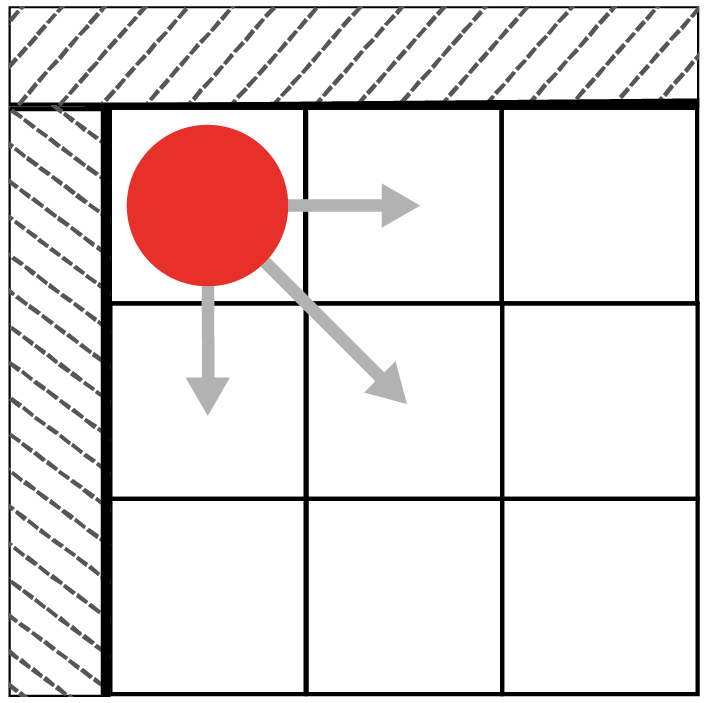
\includegraphics[width=0.33\linewidth]{pics/Kapitel_3/Kapitel_3_pic1.png}
		\captionof{figure}[3.1.1]{Ecksituation}
		\label{fig:3.1.1}
	\end{minipage}
	\vspace{1em}

    \textbf{Beispiel 2:} Liegt ein Stein am rechten Rand, so ist es möglich den Stein vertikal umzufärben, aber nicht horizontal oder schräg, wie man auf Abbildung \ref{fig:3.1.2} durch die Pfeile gut erkennen kann. Somit ist dieses Feld zu 1/4 einfärbbar und somit wichtig.\newline
    
   	\vspace{1em}
    \begin{minipage}{\linewidth}
    	\centering
    	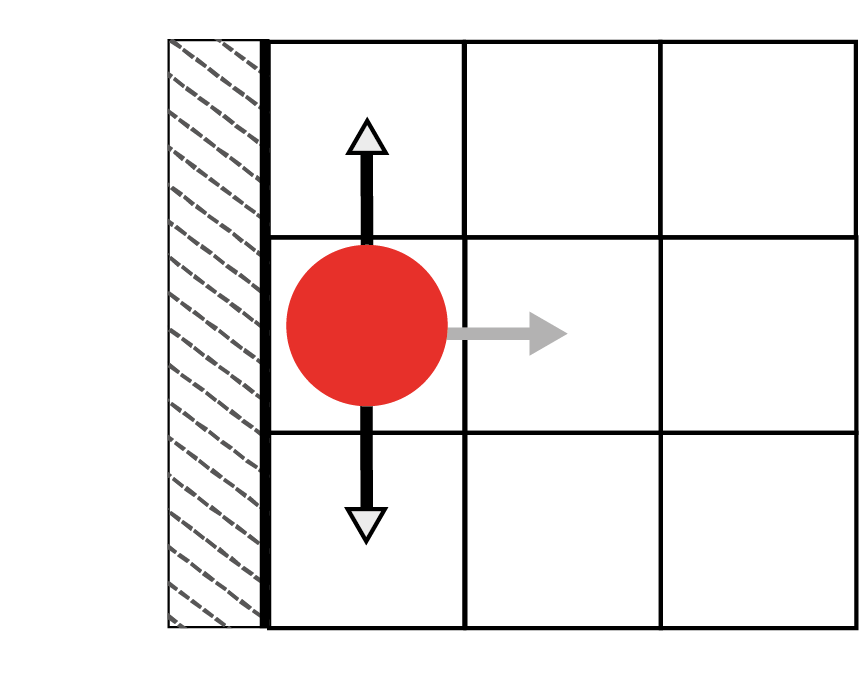
\includegraphics[width=0.33\linewidth]{pics/Kapitel_3/Kapitel_3_pic2.png}
    	\captionof{figure}[3.1.2]{Randsituation}
    	\label{fig:3.1.2}
    \end{minipage}
	\vspace{1em}

    \textbf{Beispiel 3:} Liegt ein Stein innerhalb des Spielfeldes, so ist es möglich den Stein horizontal, vertikal und schräg einzufärben. Somit ist dieses Feld zu 4/4 einfärbbar und damit nicht so wichtig. Auf Abb. \ref{fig:3.1.3} gut durch die schwarzen Pfeile zu erkennen.\newline

   	\vspace{1em}
    \begin{minipage}{\linewidth}
    	\centering
    	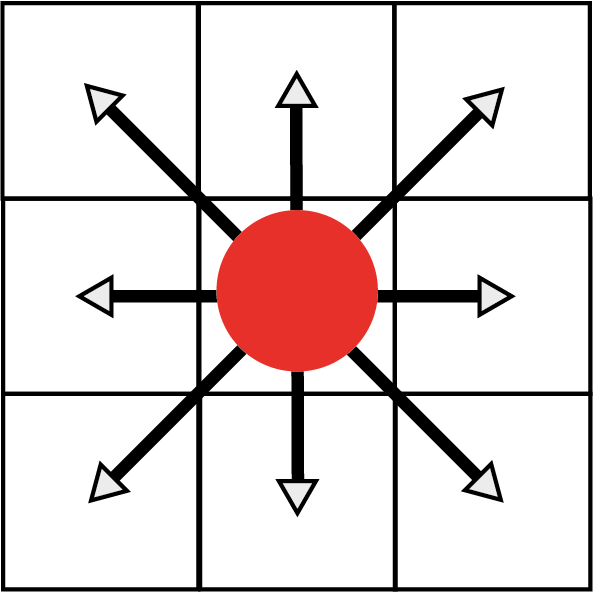
\includegraphics[width=0.33\linewidth]{pics/Kapitel_3/Kapitel_3_pic3.png}
    	\captionof{figure}[3.1.3]{Situation auf offenem Spielfeld}
    	\label{fig:3.1.3}
    \end{minipage}
	\vspace{1em}
	
    \textbf{Beispiel 4:} Wie gut auf Abb. \ref{fig:3.1.4} zu erkennen, liegt ein Stein innerhalb des Spielfeldes und zusätzlich ist links oben (Richtung 7) ein Stein der selben Farbe, der zu 0/4 einfärbbar ist, dann ist der Stein von links oben nach rechts unten und umgekehrt nicht einfärbbar. Somit ist dieses Feld zu 3/4 einfärbbar und damit wichtiger als ein Feld wie in Beispiel 3.\newline

   	\vspace{1em}
    \begin{minipage}{\linewidth}
    	\centering
    	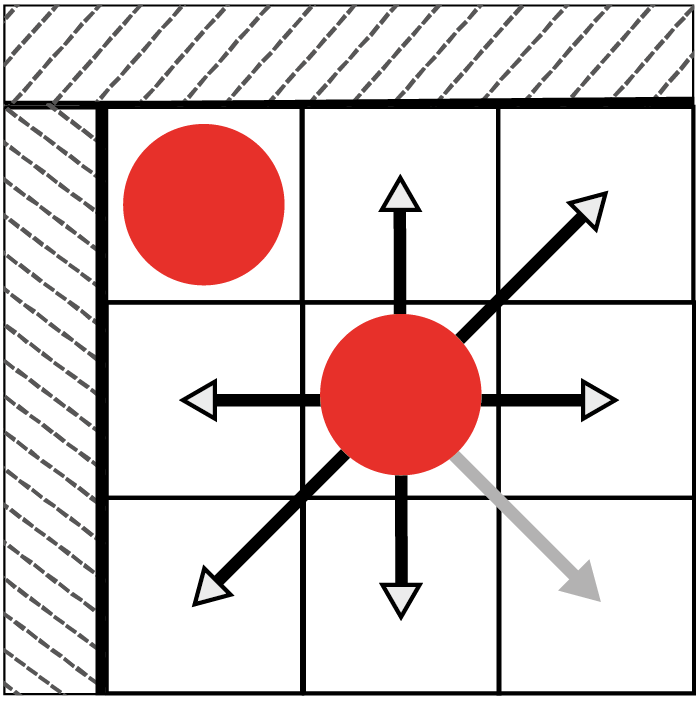
\includegraphics[width=0.33\linewidth]{pics/Kapitel_3/Kapitel_3_pic4.png}
    	\captionof{figure}[3.1.4]{Der mittlere Stein wird teils durch den Eckstein geschützt}
    	\label{fig:3.1.4}
    \end{minipage}
	\vspace{1em}
	
	Dieser Ansatz bewertet das Zusammenspiel von Spielfeldrand und den Spielsteinen untereinander und schafft damit eine hoffentlich gute Abschätzung des tatsächlichen Wertes der aktuellen Spielsituation.

    \subsection{Spielfeldbewertung: 2. Vorschlag}

    Die Idee der zweiten Spielfeldbewertung ist die eigene Mobilität einzuschätzen. Denn wenn man nur sehr wenige Möglichkeiten hat einen Zug zu machen kann der Gegner bestimmen wo man hinsetzten muss und hat selbst keinen oder nur einen geringen Einfluss auf den Spielverlauf. Im schlimmsten Fall hat man gar keine Möglichkeit zu ziehen und ermöglicht so den Gegnern mehrmals zu färben während man nichts färben kann.

    \vspace{1em}


    Hierbei ist zu beachten, dass der Sprung von einen möglichen Zug zu zwei möglichen Zügen eine größere Verbesserung ist als von 10 auf 20 mögliche Züge.
    Zu Beginn eines Spieles hat man natürlich wenig Möglichkeiten Steine zu platzieren aber der Gegner hat auch nicht so viele Möglichkeiten Stein zu platzieren, so dass es schwierig ist den anderen Spieler zu gewissen Aktionen zu bewegen da alle Spieler eingeschränkt sind.Eine besonders schlechte Situation ist es also wenn ein feindlicher Spieler viele Zugmöglichkeiten hat während man selbst nur sehr wenige hat.

    Beispiel 1: Hier hat Blau keinen Zug mehr Blau muss also aussetzen.

   	\vspace{1em}
	\begin{minipage}{\linewidth}
		\centering
		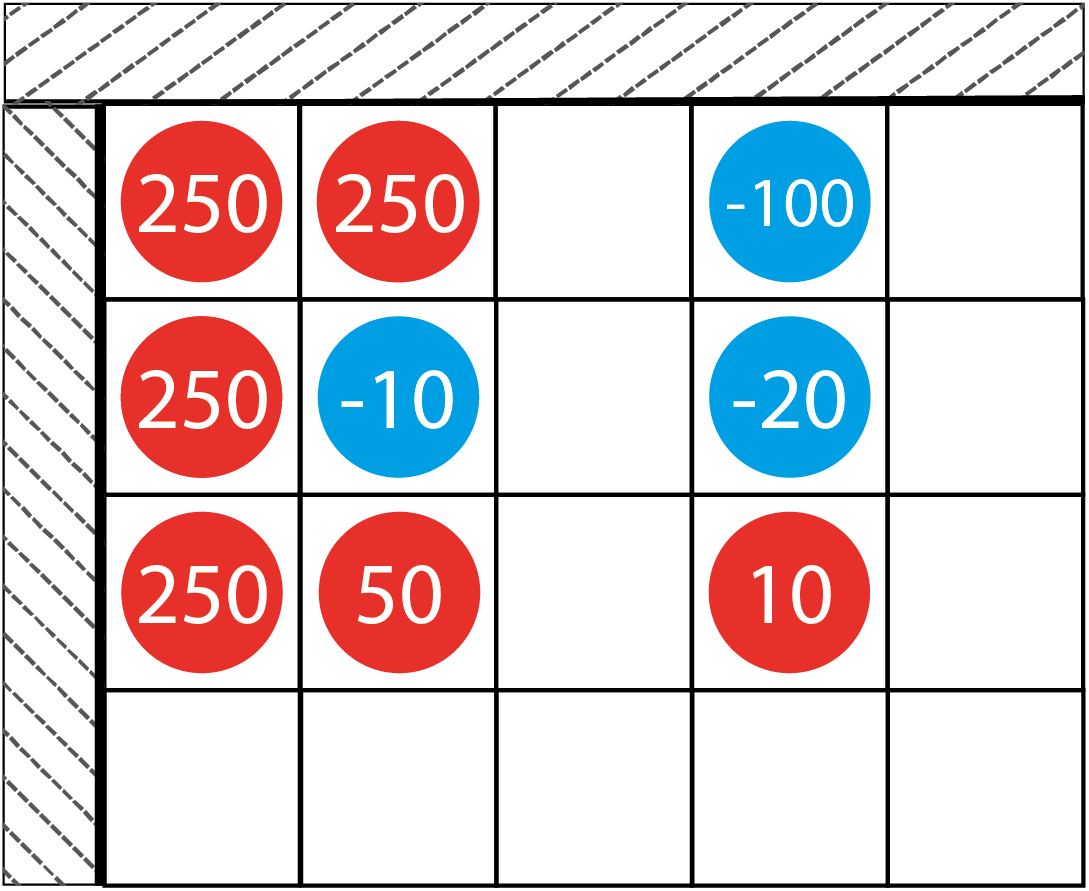
\includegraphics[width=0.33\linewidth]{pics/Kapitel_3/Kapitel_3_pic5.png}
		\captionof{figure}[3.2.1]{Situation ohne mögliche Züge für blau}
		\label{fig:3.2.1}
	\end{minipage}
	\vspace{1em}
	
    Beispiel 2: Blau hat nur einen möglichen Zug er hat also keinen Einfluss auf das Spiel mehr, da er nichts entscheiden kann.

   	\vspace{1em}
	\begin{minipage}{\linewidth}
		\centering
		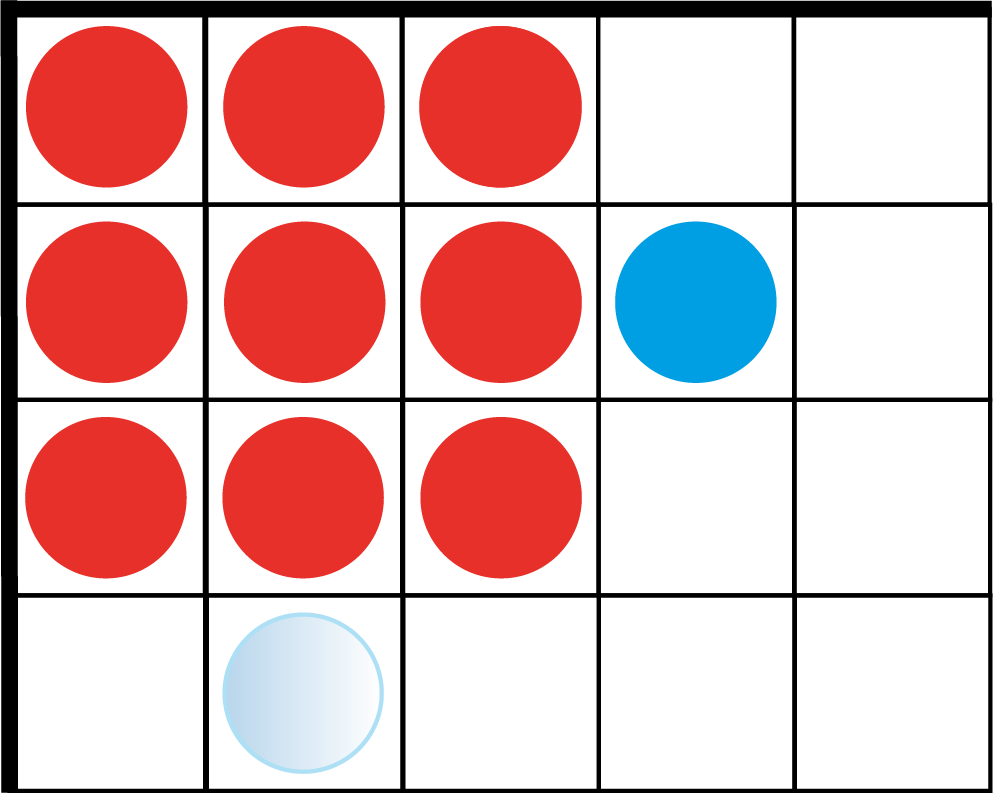
\includegraphics[width=0.33\linewidth]{pics/Kapitel_3/Kapitel_3_pic6.png}
		\captionof{figure}[3.2.2]{Bessere Situation mit einem möglichen Zug für blau (dargestellt in hellblau)}
		\label{fig:3.2.2}
	\end{minipage}
	\vspace{1em}
	
    Beispiel 3: Blau hat sehr viele Möglichkeiten Steine zu platzieren. Obwohl Rot hier mehr steine hat befindet sich blau in einer sehr guten Position da Blau deutlich mehr Zugmöglichkeiten hat als Rot.

   	\vspace{1em}
	\begin{minipage}{\linewidth}
		\centering
		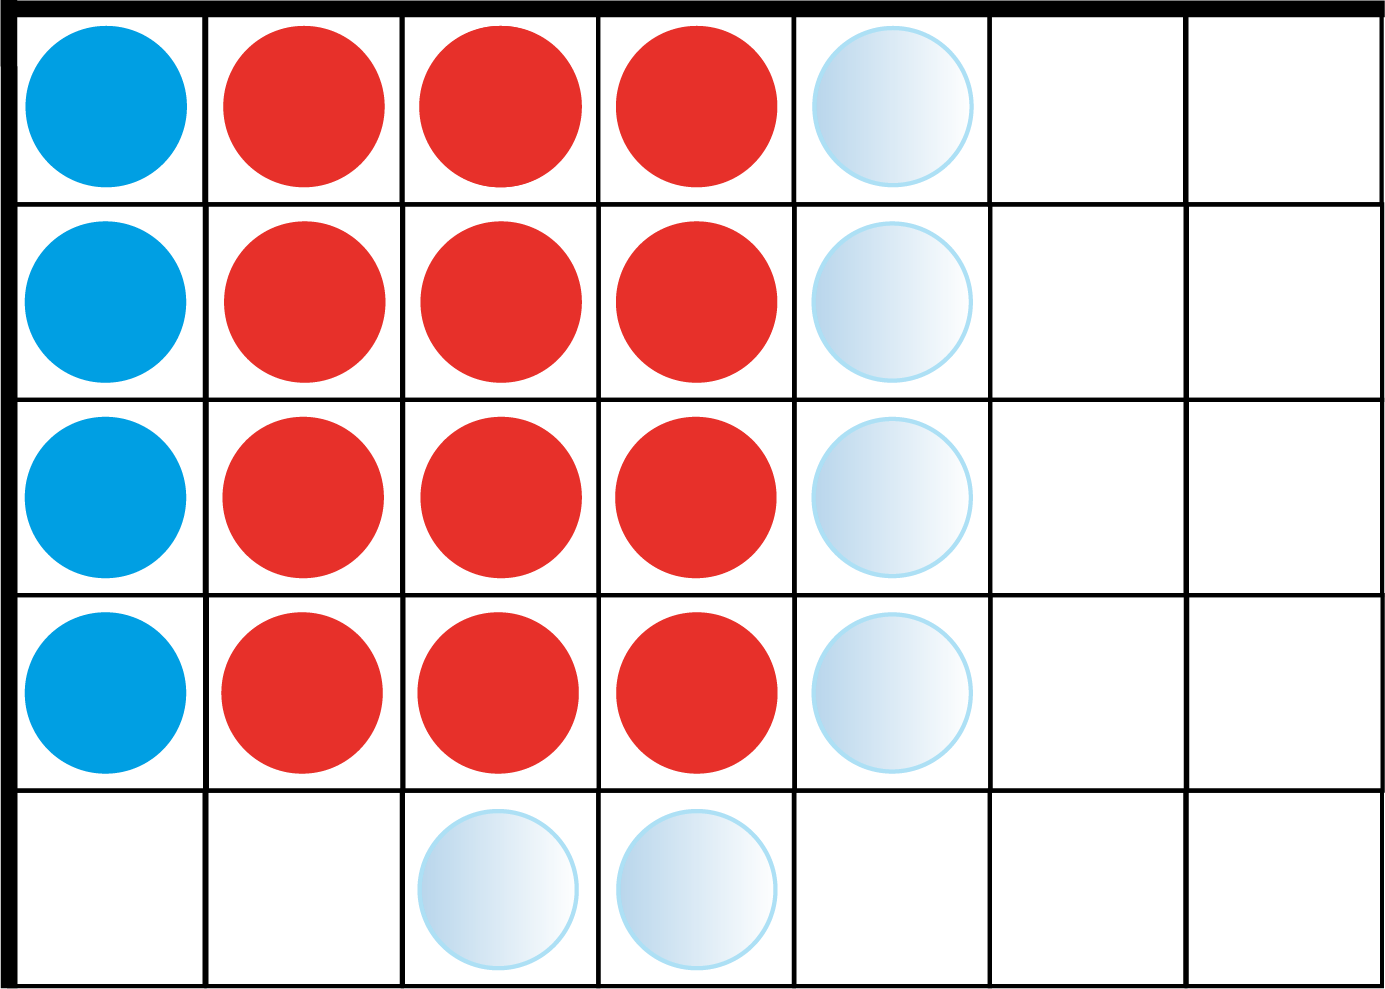
\includegraphics[width=0.33\linewidth]{pics/Kapitel_3/Kapitel_3_pic7.png}
		\captionof{figure}[3.2.3]{Ideale Situation für blau mit vielen möglichen Zügen (dargestellt in hellblau)}
		\label{fig:3.2.3}
	\end{minipage}
	\vspace{1em}
	
    Die Art der Bewertung soll verhindern, dass man die Möglichkeit verpasst gegnerische Steine zu färben.

	%TODO bei tims vorschlag abbildungsbeschreibung und ref im text benutzen
	%TODO Korrekturlesen
    \subsection{Final implementierte Spielfeldbewertung}
    \vspace{1em}
	%Beschreiben Sie abschließend, welche Heuristik final in Ihrem Client umgesetzt ist. Beschreiben Sie dazu auch Werte von Parametern (Kriterien und Gewichtungen), die Sie in den einzelnen Implementierungen nutzen. Welche statischen Vorberechnungen Sie machen, um z.B.\ das Spielfeld zu analysieren, etc.

	Nach einer Reihe unterschiedlicher Ansätze eine möglichst gute Heuristik zu konzipieren und zu implementieren, ist das Resultat eine Abwandlung des ersten Vorschlags geworden. Neben einigen anderen Überlegungen, findet ebenso das Konzept der Mobilität aus dem zweiten Vorschlag Einsatz.\\
	Wie schon im ersten Vorschlag beschrieben, ist auch hier die \glqq Färbbarkeit\grqq, auch \glqq Sicherheit\grqq{}  genannt, das Kernkonzept der Heuristik. Es gibt acht Richtungen, die aber auf vier gegenüberliegende Richtungen reduziert werden können. Durch strahlenförmiges Vorgehen, wird jede dieser acht von jedem Feld auf eben diese \glqq Sicherheit\grqq{}  überprüft. Das bedeutet z.B., dass Felder, die nicht am Rand liegen und dadurch nicht sicher sind, durch andere eigene Felder, die aber am Rand liegen geschützt werden können. Folgende Abbildung  \ref{fig:heuristik_3.3.1} soll das Konzept verdeutlichen. Rot ist die eigene KI und blau der Gegner. Die Zahlen auf den Feldern sind die durch die \glqq Sicherheit\grqq{} hergeleiteten Heuristikwerte.
	
	\vspace{1em}
	\begin{minipage}{\linewidth}
		\centering
		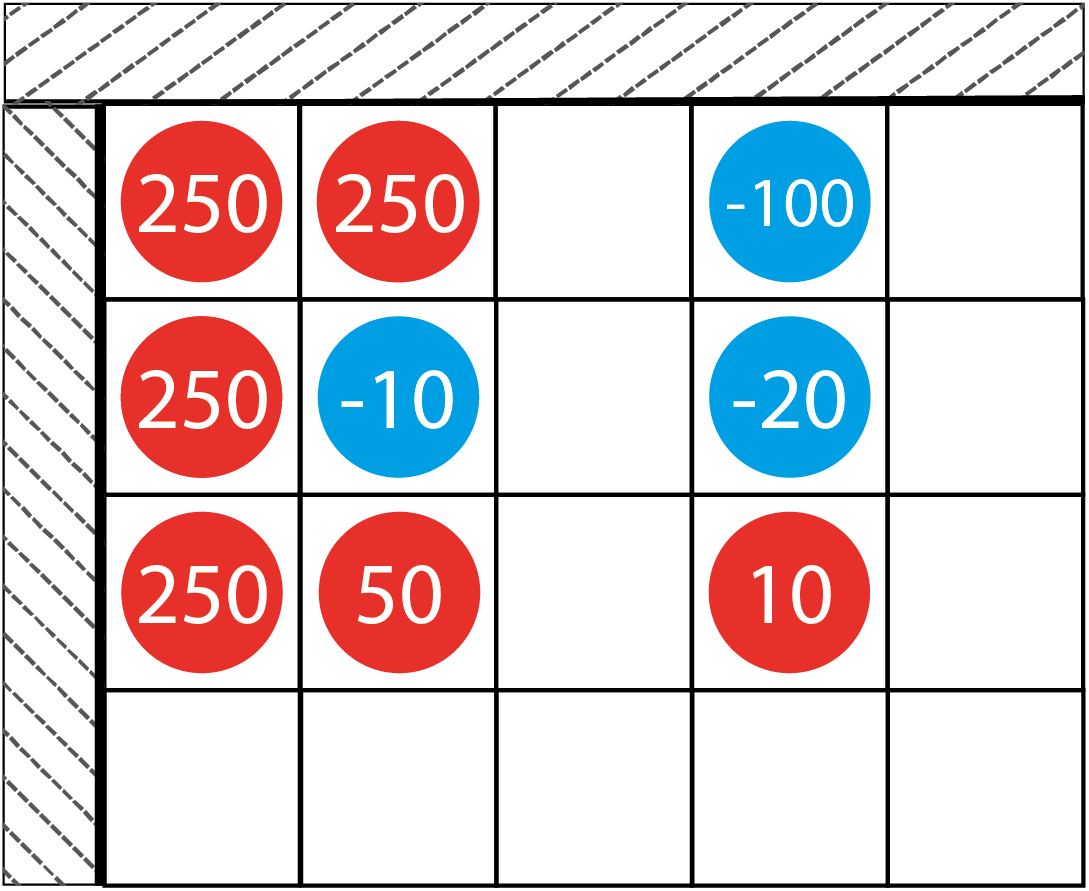
\includegraphics[width=0.4\linewidth]{pics/Kapitel_3/Kapitel_3_pic8.png}
		\captionof{figure}[Heuristik_3.3.1]{Spielsituation mit Heuristikwerten\footnotemark }
		\label{fig:heuristik_3.3.1}
	\end{minipage}
	\footnotetext{Werte: \glqq Ecke\grqq : 250, \glqq am Rand\grqq : 100,  \glqq zwei Richtungen sicher\grqq: 50, \glqq eine Richtung\grqq sicher: 20, \glqq keine Richtung\grqq sicher 10}

	Die \glqq Sicherheit\grqq{} der Felder wird für jeden Spieler berechnet. Die Heuristikwerte der Gegenspieler werden negativ der Bewertung angerechnet. So entsteht eine Karte, die das Zusammenspiel zwischen Spielern untereinander und der Randsteine beurteilt.
	
	Überschreibsteine und die Mobilität, also die Anzahl möglicher Züge, werden in dieser Heuristik bis jetzt relativ simpel bewertet. Die Anzahl der jeweiligen Variable wird mit einem Gewichtungsfaktor bewertet und auf die finale Bewertung addiert. Überschreibsteine sind für uns sehr wichtig, weswegen wir sie sehr hoch mit 1000 Punkten bewerten.
	
	Deswegen wählen wir wenn die KI auf ein Bonusfeld zieht, standardmäßig ein Überschreibstein aus, da vor allem in den letzten Zügen, ein solcher sehr viele Steine färben kann. Inversions- und Choicefelder werden anhand des durch den Tausch entstehendes Wertes beurteilt.
	
	Durch das Zusammenwirken aller Komponenten der Heuristik entsteht eine möglichst ganzheitliche Bewertung des Spielfeldes, die uns helfen soll gegen Aachen zu gewinnen.

    \newpage
    % ----------------------------------------------------------------------------------
    % Kapitel: Statistiken
    % ----------------------------------------------------------------------------------
    \section{Statistiken}
    \vspace{1em}
    %Integrieren Sie in diesen Abschnitt alle Ergebnisse von Projektaufgaben, die mit Erstellungen von Statistiken zu tun haben. Geben Sie dabei auch Diagramme an und interpretieren Sie die darin dargestellten Kurven. Beschreiben Sie zu jedem implementierten Verfahren, ob und welchen Nutzen es aus Ihrer Sicht gebracht hat.
	Dieser Abschnitt des Berichts zählt zu den wichtigsten, wenn es um den KI-Clienten selbst geht. Es werden Werte zu verschiedenen Optimierungen und Algorithmen verglichen. So kann gezeigt werden, welchen Einfluss bestimmte \grqq Verbesserungen\glqq{} haben und ob diese wirklich den Clienten kompetitiver machen. Oft denken wir, kann es sinnvoll sein, manche Optimierungen abzuschalten, da z.B. durch zu viel Overhead oder ungünstige Situationen im Spiel, die KI schlechter abschneidet. Diese und weitere Fragestellungen werden in diesem Kapitel hoffentlich beantwortet.
	%TODO - Digramme für Rechenzeit für Zustand, Anzahl Zustände, Gesamtzeit pro Zug

	%TODO - Vergleich Paranoid und alpha beta

	%TODO - Vergleich zugsortierung mit und ohne anhand Rechenzeit für Zustand, Anzahl Zustände, Gesamtzeit pro Zug and min 10 maps

	%TODO - Vergleich verschiedener Fenstergrößen für Aspiration Windows um das beste zu finden.(nicht unbedingt viel statistiken)
	
	%TODO - Vergleich Aspiration windows und alpha beta pruning mit statistiken

    \subsection{Vergleich Paranoid und Alpha-Beta Pruning}
    \vspace{1em}

    \subsection{Vergleich zwischen Zugsortierung und keine Zugsortierung}
    \vspace{1em}

    \subsection{Vergleich verschiedener Aspiration-Window-Größen}
    \vspace{1em}

	\subsection{weitere tolle vergleiche}
	\vspace{1em}

    \newpage
    % ----------------------------------------------------------------------------------
    % Kapitel: Bombenphase
    % ----------------------------------------------------------------------------------
    %TODO Korrekturlesen
    \section{Bombenphase}
    \vspace{1em}
    %Beschreiben Sie, wie Sie Bomben werfen (z.\,B.\ die eingesetzte Bewertungsheuristik und, ob Sie in die Tiefe rechnen und falls ja, wie tief Sie rechnen)
    
    Die Bombenphase ist ein wichtiger Teil des Spiels, stand für unser Team aber nicht im Vordergrund. Das kommt da her, da wir den Einfluss der Bomben auf den meisten Karten als eher gering ansehen und uns deswegen auf die gute Platzierung und den Erhalt von Überschreibsteinen fokussiert haben.\\
    Deshalb ist die Heuristik der Bombenphase sehr simpel und schnell gehalten. Die Bewertung basiert auf der trivial Heuristik und zählt die Anzahl gegnerischer Steine. Der beste Zug, also der, der die meisten der/des gegnerischen Spielsteine zerstört wird gewählt. Wenn eigene Steine dazwischen liegen wird das ignoriert. Das hat den Nachteil, dass wir in gewissen Situationen zwar möglichst viele gegnerische Felder zerbomben, aber keine Rücksicht bei unseren Steinen nehmen und wenn wir es optimal implementiert hätten, ein paar Steine besser wären. Dadurch, dass wir gefundene Bombenzüge immer vorne an unsere Liste anhängen, bleibt am Schluss nach einer Sortierung nach maximaler Anzahl der gegnerischen Felder, der letzte gefundene Wert ganz vorne. Dieser wird nun gewählt und und ist möglicherweise nicht optimal.\\
    Wie anfangs aber erwähnt, haben wir unseren Fokus jedoch anders gelegt. Die folgenden zwei Beispiele zeigen einen \glqq Standardfall\grqq{} und einen Fall bei dem der eben genannte Nachteil zum Vorschein tritt.

	\vspace{1em}
	\begin{minipage}{\linewidth}
		\centering
		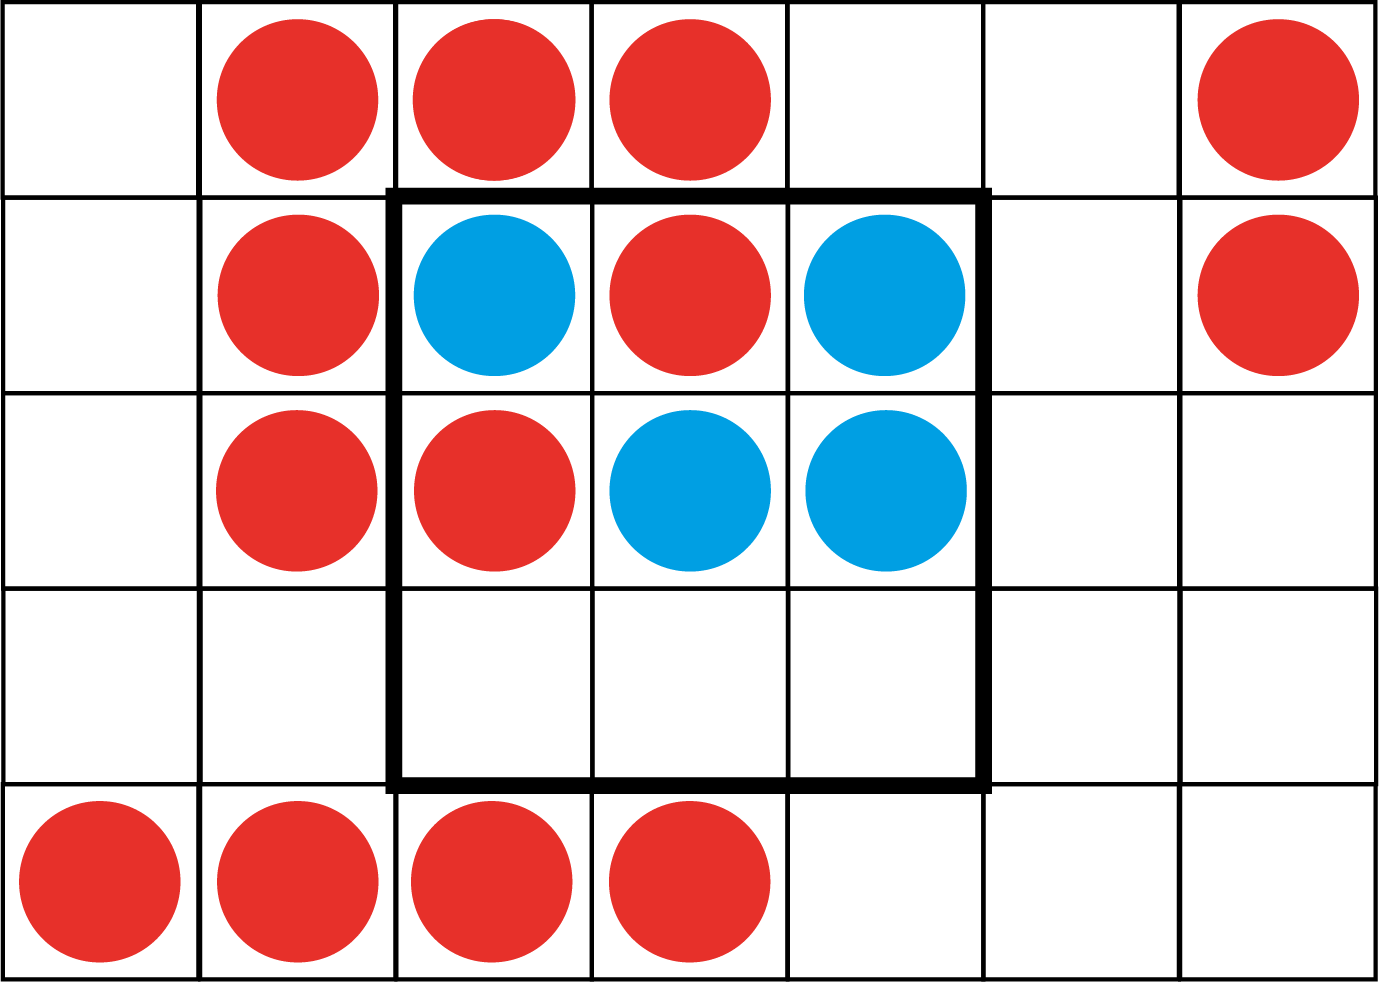
\includegraphics[width=0.6\linewidth]{pics/Kapitel_5/Kapitel_5_pic1.png}
		\captionof{figure}[bomben1]{\glqq Standardfall\grqq{} bei Bombenstärke 1}
		\label{fig:bomben1}
	\end{minipage}
	\vspace{1em}
	
	Der oben in Abbildung \ref{fig:bomben1} gezeigte Fall zeigt, mehr oder weniger was normalerweise passiert. Die KI wählt einen Zug (dicker schwarzer Rahmen), der möglichst viele gegnerische Steine umfasst, trifft dabei notwendigerweise einige unserer Steine.

	
	\vspace{1em}
	\begin{minipage}{\linewidth}
		\centering
		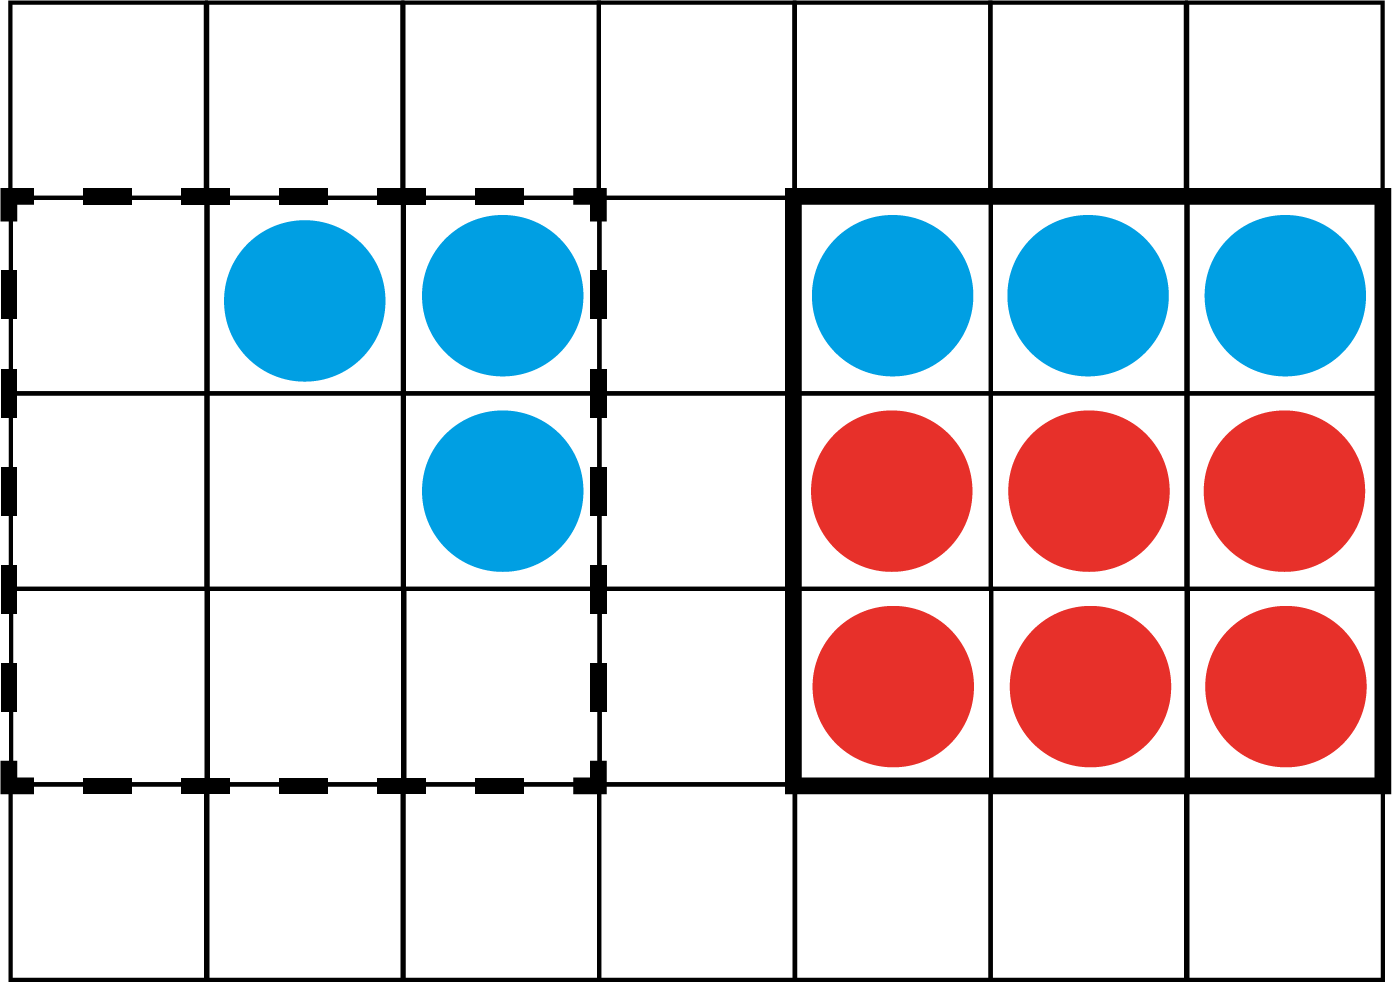
\includegraphics[width=0.6\linewidth]{pics/Kapitel_5/Kapitel_5_pic2.png}
		\captionof{figure}[bomben2]{Sonderfall mit Nachteilen bei Bombenstärke 1}
		\label{fig:bomben2}
	\end{minipage}
	\vspace{1em}
	
	In diesem Fall wie auf Abbildung \ref{fig:bomben2} jedoch wählt die KI den falschen Zug, da aufgrund der Sortierung der speichernden Liste der letzte maximale Zug (dicker Rahmen) realisiert wird. Der eigentlich beste Zug (gestrichelter Rahmen) wird in dieser Runde so nicht getätigt.
	
	Insgesamt funktioniert unsere Implementierung zur Bombenphase gut, jedoch nicht optimal. Bis zum finalen Spiel können wir hoffentlich noch einige Verbesserungen daran vornehmen.

    
    % ----------------------------------------------------------------------------------
    % Kapitel: Eigene Spielfelder
    % ----------------------------------------------------------------------------------
    \section{Wettbewerbs-Spielfelder}
    \vspace{1em}
    %Beschreiben Sie in diesem Abschnitt die Spielfelder, die Sie für den Wettbewerb eingereicht haben/einreichen wollen. Fügen Sie in diesen Abschnitt auch die entsprechenden Bilder der Karten ein, geben Sie Zusatzinformationen wie Spieleranzahl, Bombenanzahl und -stärke, Anzahl Überschreibsteine etc.\ an.

    %Beschreiben Sie außerdem, warum sie die jeweiligen Karten eingereicht haben: in welcher Hinsicht versprechen Sie sich von den eingereichten Karten Vorteile; in wie weit sind diese Karten auf Ihren Client und die darin implementierte Heuristik zugeschnitten, etc.
	%TODO Karten erstellen und wie oben beschreiben
	Als 2-Spielermap haben wir einen kleine Karte bestehend aus zwei Pixel-Art Figuren ausgewählt. Die Figuren stellen einen Creeper und ein Skellet aus dem Spiel Minecraft da. Außerdem sind die Figuren mit einigen Transitionen verbunden. Im Skellett befinden sich noch vier Choice-Steine.
	
	Unsere 4-Spielermap ist eine große Karte mit einem kleinen Tannenbaum in der Mitte. Da unsere KI auf großen Karten mit einigen Überschreibsteinen besonders gut zu sein scheint haben wir versucht das mit dieser Karte umzusetzen.
	
	% ----------------------------------------------------------------------------------
	% Kapitel: Anforderungen an einen Reversi-Replayer
	% ----------------------------------------------------------------------------------
	\section{Anforderungen an einen Reversi-Replayer}
	\vspace{1em}
	%TODO Korrekturlesen
	%Stellen Sie in der Gruppe eine Liste von mindestens f¨unf unterschiedlichen Anforderungen an einen Reversi-Replayer bzw. an das von Herrn Krapfl (Bachelorand) vorgestellte Tool zusammen.
	
	In diesem Kapitel geht es um Ideen zu Features, für einen ReversiXT-Replayer. Wir hoffen, dass dadurch zukünftige ReversiXT-Generationen bessere Clienten programmieren können und sich beim Fehlerfinden leichter tun.
	
	\textbf{Anforderung 1:} Ein Spiel sollte von Anfang bis Ende vorwärts und rückwärts schrittweise durchgehbar sein. Dabei sollen alle Daten wie Bomben, Überschreibsteine, Punkte usw. aktuell gehalten werden.
	
	\textbf{Anforderung 2:} Eine weitere Idee ist es, die Standardausgabe jedes Clienten sichtbar zu machen und diese auch schrittweise nachvollziehbar zu machen. Das würde das Debugging erleichtern und den Gruppen die Möglichkeit geben, durch übersichtliche Ausgaben den Ablauf des Spiels Verständlicher zu machen.
	
	\textbf{Anforderung 3:} Den Gruppen durch ein Interface erlauben, online eigene Spiele mit eigenen Parametern wie Tiefe und Zeit zu starten. Dort sollen die Spieler außerdem ihre Gegner und die Karte auf der gespielt werden soll ausgewählt werden. Natürlich muss das Testen durch eine Art Kontingentsystem limitiert sein, dass die Gruppen das Spielsystem nicht ausnützen können. 
	
	\textbf{Anforderung 4:} Eine Profilsystem würde sich anbieten. In diesem System werden alle vergangenen Spiele gespeichert. Ein Vergleichsfeature macht es möglich Spiele miteinander zu vergleichen. Z.B Spiele auf der gleichen Karte gegen den gleichen Gegner könnte man über den Verlauf des Semesters vergleichen und so eine Verbesserung/Verschlechterung feststellen.
	
	\textbf{Anforderung 5:} Als Erweiterung der Anforderung 3 \& 4 könnte man dem System zusätzlich zu Karte und Gegner, Parameter für den eigenen Clienten mitgeben, z.B. verschiedene Werte um die Heuristik zu testen. Im Zusammenspielt mit dem Vergleichsfeature und vielen Spielen könnte man so ein gutes Tool bauen um optimale Werte für Heuristik, aspiration windows und iterative deepening zu finden.
	
	Insgesamt ist der Replayer eine super Idee, um die Teams bei der Fehlerfindung und der Verbesserung ihrer KI-Clienten zu unterstützen. Wir hoffen Herr Krapfl kann aus unseren Vorschäge für seine Bachelorarbeit nützliche Ideen ziehen.
	
    \newpage
    % ----------------------------------------------------------------------------------
    % Kapitel: Fazit
    % ----------------------------------------------------------------------------------
    \section{Fazit}
    \vspace{1em}
    %Beschreiben Sie in diesem Abschnitt u.a.\ was Ihnen an diesem Fach gefallen hat und welche Verbesserungsvorschläge Sie für künftige Veranstaltungen haben. Was konnten Sie dazulernen, in welchen Bereichen haben Sie sich verbessert. Welche Problemsituationen gab es während der Projekterstellung, wie sind Sie diese angegangen und wie haben Sie diese gelöst. Was haben Sie evtl.\ vermisst.
	Die Vorfreude in unserem Team auf diese Projekt war groß. Die Vorstellung, ein eigenes Projekt von Anfang bis Ende zu gestalten, hat alle motiviert. Am Ende des Semesters angekommen, kann man sagen, dass Vorstellung und Realität sich aber doch sehr von einander unterscheiden. In der Überlegung ist immer alles einfacher und funktioniert problemloser. In der Realität komm es aber doch immer anders. Im Verlauf der Zeit, sind wir auf Probleme, fachspezifischer aber auch menschlicher Art, gestoßen die uns auf die Probe gestellt haben. Vor allem in der mittleren Phase haben uns viel nervenaufreibende Bugs geplagt und teilweise schien nichts mehr zu funktionieren. Dazu hatten wir Probleme eine gute Heuristik zu erstellen und mussten diese mehrfach neu konzipieren und programmieren. Aber gerade durch diese schwierigere Zeit haben wir gelernt nicht aufzuhören und am nächsten Tag nochmal strukturiert das Problem zu analysieren. Auch unsere Programmierfähigkeiten haben sich dadurch verbessert. Vor allem haben wir viel für den späteren Berufsalltag gelernt denke ich. Dort sind Deadlines und Bugs an der Tagesordnung und es gilt diese möglichst stressfrei und strukturiert zu bearbeiten.\\
	Insgesamt kann man sagen, dass wir mehr mitgenommen haben als anfangs gedacht und das vor allem aus verschiedenen unerwarteten Bereichen. Das ist einer der Gründe warum uns \grqq ZOCK\glqq{} gut gefallen hat. Ein weiterer ist der Wettbewerbsgedanke unter den Teams und Aachen. Auch Herr Kern selbst, der durch konstruktive Kritik alle immer \glqq auf zack\grqq{} hält, hat dazu beigetragen, dass es auch Spass macht. So war die Motivation trotz zwischenzeitlichen Schwierigkeiten hoch.\\
	Die Ergebnisse des Projekts können sich auch sehen lassen. Die KI wird nicht mehr disqualifiziert und erreicht gute Punktewerte. Zum Zeitpunkt der Abgabe dieses Berichts haben wir noch Ideen zur Verbesserung der Heuristik und hoffen diese bis zum großen Endspiel noch umsetzten zu können. Es geht dabei darum mehr Überschreibsteine zu erspielen, da wir diese oft für spielentscheidend halten.\\
	Allgemein schien mir das Fach gut durchdacht und erprobt. Deswegen haben wir nur einen Verbesserungsvorschlag. Die Deadline für die Abgabe des Projektberichts sollte etwas früher sein. Dadurch entstehen bei schlechtem Zeitmanagement weniger, Interessenskonflikte zwischen für die Prüfungen lernen und den Bericht fertig schreiben.\\
	Abschließend können wir \glqq ZOCK \grqq{} früheren Semestern nur empfehlen. Wir haben einiges gelernt und hatten viel Spass. Wer gern etwas mehr Zeit als bei anderen Fächern investieren möchte, dafür aber viel mitnehmen will ist hier genau richtig.
	 %TODO Hier weiter machen

    \newpage
    
    
    %TODO - Folgenden Teil vor Abgabe löschen!!!!!
    % ----------------------------------------------------------------------------------
    % Kleine Einführung in LaTeX-Elemente
    % ----------------------------------------------------------------------------------
    \section{\LaTeX-Elemente}
    Dieser Abschnitt soll nicht Bestandteil des Projektberichtes sein, sondern beinhaltet lediglich einige Informationen über \LaTeX-Distributionen, Editoren und \LaTeX-Elemente, die Ihnen beim Einstieg in das \LaTeX-Textsatzsystem helfen sollen.

    \subsection{\LaTeX-Distributionen nach Betriebssystemen}

    \subsubsection{\LaTeX-Distributionen}
    Folgende Haupt-\LaTeX-Distributionen stehen Ihnen zur Verfügung:
    \begin{itemize}
        \item Windows:\quad \texttt{MiKTeX}\quad Webseite:\quad\url{http://www.miktex.org}
        \item Linux/Unix:\quad \texttt{TeX Live}\quad Webseite:\quad\url{http://tug.org/texlive/}
        \item Mac OS:\quad \texttt{MacTeX}\quad Webseite:\quad\url{http://www.tug.org/mactex/}
    \end{itemize}

    \subsubsection{\LaTeX-Editoren}
    Auf folgenden Webseiten können Sie einige hilfreiche \LaTeX-Editoren finden:
    \begin{itemize}
        \item Windows/Linux/Mac OS: \url{http://www.xm1math.net/texmaker/}
        \item Windiws: \url{http://www.texniccenter.org/}
        \item Mac OS: \url{http://pages.uoregon.edu/koch/texshop/}
    \end{itemize}

    Falls bei den oben genannten Editoren kein passender vorhanden war, findet sich auf Wikipedia eine Zusammenstellung vieler weiterer \LaTeX-Editoren:\\[1em]
    \hspace*{3cm}\url{https://en.wikipedia.org/wiki/Comparison_of_TeX_editors}


    \subsection{Unterabschnitt}
    Zum Einfügen eines Bildes, siehe Abbildung \ref{fig:reversi01}, wird die \textit{minipage}-Umgebung genutzt, da die Bilder so gut positioniert werden können.

    \vspace{1em}
    \begin{minipage}{\linewidth}
        \centering
        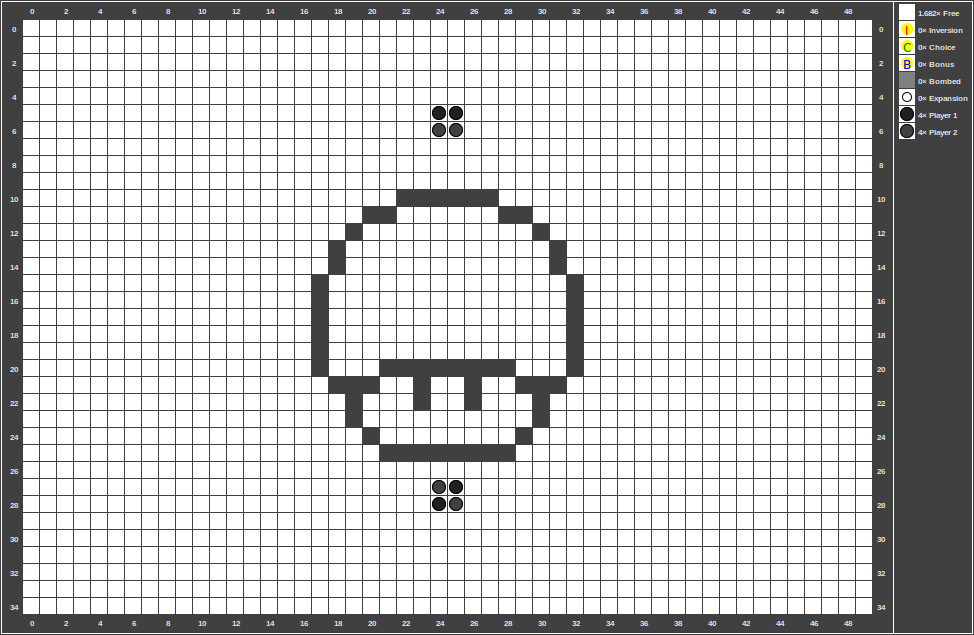
\includegraphics[width=0.6\linewidth]{pics/gamefield01.png}
        \captionof{figure}[Spielfeld 01]{Unbespieltes Spielfeld\footnotemark }
        \label{fig:reversi01}
    \end{minipage}
    \footnotetext{Diesem Spielfeld wurden noch keine Spieler zugewiesen (daher die dunklen Spielsteine)}

    Nachdem das Spielt gestartet wurde und beiden Spielphasen durchlaufen wurden, siegt schließlich der Spieler mit der Farbe rot.

    \vspace{1em}
    \begin{minipage}{\linewidth}
        \centering
        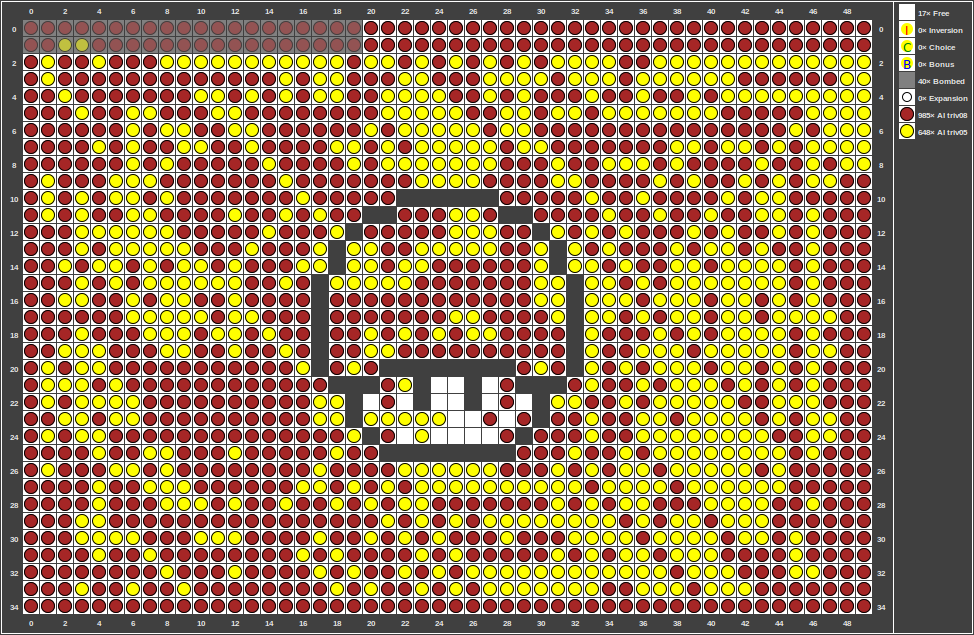
\includegraphics[width=0.6\linewidth]{pics/gamefield02.png}
        \captionof{figure}[Spielfeld 02]{Finales Spielfeld\footnotemark }
        \label{fig:reversi2}
    \end{minipage}
    \footnotetext{Das Spielfeld nach der Zug- und Bombenphase. Spieler rot gewinnt eindeutig.}
    
    \begin{wrapfigure}{r}{0.25\textwidth}
    	\centering
    	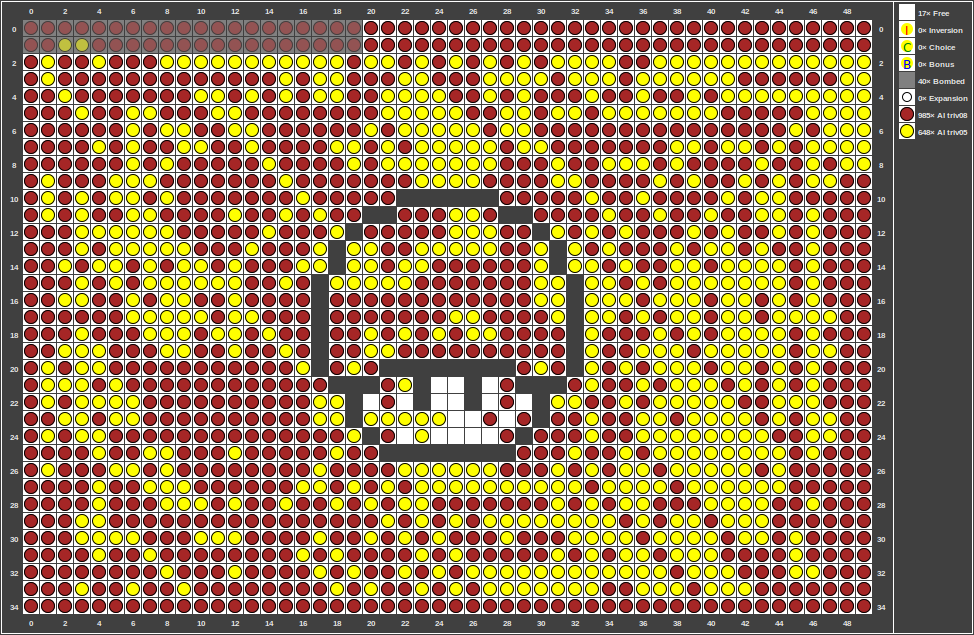
\includegraphics[width=0.25\textwidth]{pics/gamefield02.png}
    	\caption{kleines Bild}
    	\label{fig:test11111111111111}
    \end{wrapfigure}
Toller Text nebem dem rechts ein Tolles Bild ist. Toller Text nebem dem rechts ein Tolles Bild ist. Toller Text nebem dem rechts ein Tolles Bild ist. Toller Text nebem dem rechts ein Tolles Bild ist. Toller Text nebem dem rechts ein Tolles Bild ist.
    \subsection{Tabellen}
    In diesem Abschnitt wird eine Tabelle (siehe Tabelle \ref{tab:beispiel}) dargestellt.

    \vspace{1em}
    \begin{table}[!h]
        \centering
        \begin{tabular}{|l|l|l|}
            \hline
            \textbf{Name} & \textbf{Name} & \textbf{Name}\\
            \hline
            1 & 2 & 3\\
            \hline
            4 & 5 & 6\\
            \hline
            7 & 8 & 9\\
            \hline
        \end{tabular}
        \caption{Beispieltabelle}
        \label{tab:beispiel}
    \end{table}


    \subsection{Auflistung}
    Für Auflistungen wird die \textit{enumerate}- oder \textit{itemize}-Umgebung genutzt.

    \begin{itemize}
        \item Nur
        \item ein
        \item Beispiel.
    \end{itemize}

    \subsection{Listings}
    Zuletzt ein Beispiel für ein Listing, in dem Quellcode eingebunden werden kann, siehe Listing \ref{lst:arduino}.

    \vspace{1em}
    \begin{lstlisting}[caption=Arduino Beispielprogramm, label=lst:arduino]
        int ledPin = 13;
        void setup() {
        pinMode(ledPin, OUTPUT);
        }
        void loop() {
        digitalWrite(ledPin, HIGH);
        delay(500);
        digitalWrite(ledPin, LOW);
        delay(500);
        }
    \end{lstlisting}

    \subsection{Tipps}
    Die Quellen befinden sich in der Datei \textit{quellen.bib}. Eine Buch- und eine Online-Quelle sind beispielhaft eingefügt. [Vgl. \cite{buch}, \cite{online}]

    \pagebreak

    % ----------------------------------------------------------------------------------------------------------
    % Kapitel
    % ----------------------------------------------------------------------------------------------------------
    \section{Kapitel}
    Lorem ipsum dolor sit amet.

    \subsection{Unterkapitel}
    Lorem ipsum dolor sit amet, consetetur sadipscing elitr, sed diam nonumy eirmod tempor invidunt ut labore et dolore magna aliquyam erat, sed diam voluptua. At vero eos et accusam et justo duo dolores et ea rebum. Stet clita kasd gubergren, no sea takimata sanctus est Lorem ipsum dolor sit amet. Lorem ipsum dolor sit amet, consetetur sadipscing elitr, sed diam nonumy eirmod tempor invidunt ut labore et dolore magna aliquyam erat, sed diam voluptua. At vero eos et accusam et justo duo dolores et ea rebum. Stet clita kasd gubergren, no sea takimata sanctus est Lorem ipsum dolor sit amet.

    \subsection{Unterkapitel}
    Lorem ipsum dolor sit amet, consetetur sadipscing elitr, sed diam nonumy eirmod tempor invidunt ut labore et dolore magna aliquyam erat, sed diam voluptua. At vero eos et accusam et justo duo dolores et ea rebum. Stet clita kasd gubergren, no sea takimata sanctus est Lorem ipsum dolor sit amet. Lorem ipsum dolor sit amet, consetetur sadipscing elitr, sed diam nonumy eirmod tempor invidunt ut labore et dolore magna aliquyam erat, sed diam voluptua. At vero eos et accusam et justo duo dolores et ea rebum. Stet clita kasd gubergren, no sea takimata sanctus est Lorem ipsum dolor sit amet.
    \pagebreak

    % ----------------------------------------------------------------------------------------------------------
    % Literatur
    % ----------------------------------------------------------------------------------------------------------
    \renewcommand\refname{Quellenverzeichnis}
    \bibliographystyle{alpha}
    \bibliography{quellen}
    \pagebreak

    % ----------------------------------------------------------------------------------------------------------
    % Anhang
    % ----------------------------------------------------------------------------------------------------------
    \pagenumbering{Roman}
    \setcounter{page}{1}
    \lhead{Anhang \thesection}

    \begin{appendix}
        \section*{Anhang}
        \phantomsection
        \addcontentsline{toc}{section}{Anhang}
        \addtocontents{toc}{\vspace{-0.5em}}

        \section{GUI}
        Ein toller Anhang.

        \subsection*{Screenshot}
        \label{app:screenshot}
        Unterkategorie, die nicht im Inhaltsverzeichnis auftaucht.

    \end{appendix}


\end{document}
